\documentclass[a4paper, 12pt]{article}

\usepackage[francais]{babel}
\usepackage{color}
\usepackage[T1]{fontenc}
\usepackage[utf8]{inputenc} %%% Encodage Unix
\usepackage{layout}
\usepackage[top=1.5cm, bottom=1.5cm, left=1.5cm, right=1.5cm]{geometry} %%% Règle la marge
\usepackage{setspace} %%% Utiliser Vspace
\usepackage{graphicx} %%% Importer images
\usepackage{pst-all,pst-eucl}
\usepackage{titlesec}
\usepackage{titletoc}
\usepackage{calc} %%% Symboles mathématiques
\usepackage{listings}
\usepackage{wasysym} %%% Symboles spéciaux (téléphone)
\usepackage{multicol}
\usepackage{lipsum}

% ----------------------------------------
% FONCTIONS
% ----------------------------------------

% Style des parties: titre encadré + nom de partie dans le cadre
\titleformat{\part}[frame]
{\normalsize}%
{\filright\sffamily\Large%
\enspace Partie \thepart\enspace}%
{8pt}
{\rule{0pt}{30pt}\sffamily\LARGE\bfseries\filcenter}

% Ajoute \tocless{} devant un \part --> pas dans la TOC
\newcommand{\nocontentsline}[3]{}
\newcommand{\tocless}[2]{\bgroup\let\addcontentsline=\nocontentsline#1{#2}\egroup}

\begin{document}
\begin{onehalfspace}

% ----------------------------------------
% PAGE DE GARDE
% ----------------------------------------

\begin{titlepage}
  \centering
      \large\textsc{Université Blaise Pascal - Clermont-Ferrand II}\\
      \textsc{UFR Sciences et Technologies}\\
    \vspace{1.5cm}
      
\includegraphics[width=0.22\textwidth]{pic_Data/blaisepascal.png}
      \hfill
      
\includegraphics[width=0.33\textwidth]{pic_Data/inra.jpg}\\
    \vspace{1.2cm}
      \large\textbf{03 septembre 2014\\
       \rule{10cm}{0.2pt}\\
       Master I Biologie et Environnement\\
       Génomique, Ecophysiologie et Production Végétales}\\
       \rule{10cm}{0.2pt}\\
    \vspace{2.5cm}
       {\LARGE\textbf{Étude du paysage transpositionnel chez le blé.\\ Re-séquençage et analyse de 45 lignées.}}\\
    \vspace{2cm}
        \LARGE{Emeric \bsc{Dynomant}} \\
    \vspace{3.5cm}
	\large\textbf{Membres du jury:}\\
	Julie \bsc{Boudet}\\
	Patricia \bsc{Drevet}\\
	Aurélie \bsc{Gousset}\\
    \vspace{2cm}
\end{titlepage}

% ----------------------------------------
% QR_CODE
% ----------------------------------------

\newpage
\thispagestyle{empty}
\begin{center}
~\vfill

\includegraphics[width=0.35\textwidth]{pic_Data/QRcode.png}\\
\vfill
\end{center}

% ----------------------------------------
% PAGE DE PRÉSENTATION
% ----------------------------------------

\newpage
\thispagestyle{empty}
\begin{center}
  
\includegraphics[width=0.35\textwidth]{pic_Data/inra.jpg}\\
\vspace{3cm}

\includegraphics[width=0.95\textwidth]{pic_Data/log_gdec.png}\\
\vspace{1.5cm}
	\large\textbf{UMR 1095 - Génétique, Diversité, Écophysiologie des Céréales (\bsc{GDEC})\\
	Équipe Structure et Évolution du Génome de Blé (\bsc{SEVEN})}\\
	5, chemin de Beaulieu\\
	63039 Clermont-Ferrand Cedex 2\\
	\phone ~ 04 73 62 43 21\\
\vspace{3cm}
	\large\textbf{Encadrants:}\\
	Frédéric \bsc{Choulet}\\
	Josquin \bsc{Daron}\\
	Étienne \bsc{Paux} \\
\end{center}


% ----------------------------------------
% PB
% ----------------------------------------
\newpage
\thispagestyle{empty}
\null

% ----------------------------------------
% RÉSUMÉ
% ----------------------------------------

\newpage
\thispagestyle{empty}
\parindent=1.5cm
\tocless{\part*{Résumé / Abstract}}

L'étude réalisée au cours de ce stage visait à caractériser l'ampleur de la variabilité génomique inter et intra-spécifique chez les \textit{Triticeae} via la mise en évidence des variations structurales dues aux éléments transposables (ET), qui représentent 85\% du génome. Une méthode bioinformatique d'analyse de séquences permettant d'identifier le polymorphisme dans la fraction répétée du génome a été développée en utilisant 237 777 extrémités d'ET comme marqueurs ISBP (Insertion Site-Based Polymorphism), identifiés le long de la séquence du chromosome 3B de la variété de référence \textit{Chinese Spring}. Une analyse de la présence/absence de chacun de ces marqueurs a ainsi été réalisée par re-séquençage du chromosome 3B de 45 variétés de blé tétra ou hexaploïdes choisies pour maximiser la diversité parmi les \textit{Triticeae}.

Les résultats obtenus ont permis de caractériser le polymorphisme à un très fort niveau de résolution. Il a également été démontré que les régions distales du chromosome sont beaucoup plus polymorphes que la région centrale. Par ailleurs, ces données ont permis de générer un dendrogramme des 45 accessions, qui est fiable au regard du niveau de ploïdie et de l'origine géographique. Enfin, il a été possible d'identifier 249 événements de transposition d'ET très récents chez \textit{Chinese Spring}, à raison de 62\% de rétrotransposons et 38\% de transposons à ADN, préférentiellement dans les régions distales.

\begin{flushright}
\underline{Mots clés} : bioinformatique, blé, éléments transposables, génome, marqueurs ISBP, phylogénie, variation de présence/absence.
\end{flushright}
\vspace{0.5cm}

This study aimed at deciphering the extent of inter and intra-specific genomic variability among the \textit{Triticeae} through the identification of structural variations due to transposable elements (TE) that represent 85\% of the genome. A bioinformatics method was established to identify polymorphism in the repeated fraction of the genome sequence by using 237 777 TE extremities as ISBP markers (Insertion Site-Based Polymorphism) annotated along the full sequence of the 3B chromosome from the reference variety \textit{Chinese Spring}. A presence/absence analysis of each marker was performed by using resequencing data of chromosome 3B from 45 tetra and hexaploid wheat accessions selected to maximize the diversity among the \textit{Triticeae}.

The results allowed characterizing polymorphism at a very high-resolution level. This approach showed that the distal regions exhibit a higher rate of polymorphism than the central region of the chromosome. In addition, these data were used to build a dendrogram of the 45 accessions, that is reliable according to ploidy level and geographic origin. This study allowed us to identify 249 very recent events of TE insertion in \textit{Chinese Spring}, involving 62\% of retrotransposons and 38\% of DNA transposons, preferentially in the distal regions.

\begin{flushright}
\underline{Keywords} : bioinformatic, genom, ISBP markers, transposables elements, presence/absence variation, phylogeny, wheat.
\end{flushright}

% ----------------------------------------
% ABRÉVIATIONS
% ----------------------------------------

\newpage
\thispagestyle{empty}
\tocless{\part*{Abréviations}}
~\\
\parindent=0cm

ADN(c): Acide Desoxyribo Nucléique (complémentaire)\\
ARN(m) : Acide Ribo Nucléique (messager)\\
BAC: Bacterial Artificial Chromosome\\
BDD: Base De Données\\
BLAST: Basic Local Alignement Search Tool\\
ET: Elément(s) Transposable(s)\\
Gb: Giga bases (1.10$^{9}$ paires de bases)\\
ISBP: Insertion Site-Based Polymorphism\\
LTR: Long Terminal Repeat\\
Mb: Mega bases (1.10$^{6}$ paires de bases)\\
MTP: Minimum Tiling Path\\
NGS: Next Generation Sequencing\\
nu: Nucléotide\\
pb: Paire de Bases\\
PCR: Polymerase Chain Reaction\\
SNP: Single Nucleotide Polymorphism\\
WGA: Whole Genome Amplification\\

% ----------------------------------------
% TABLE DES MATIÈRES
% ----------------------------------------

\newpage
\thispagestyle{empty}
\parindent=1.5cm
%%% Sommaire avec 5% d'espacement en moins interligne
{\setlength{\baselineskip}{0.95\baselineskip}
\tableofcontents\par}

% ----------------------------------------
% PB
% ----------------------------------------
\newpage
\thispagestyle{empty}
\null

% ----------------------------------------
% INTRODUCTION
% ----------------------------------------

\newpage
\setcounter{page}{1}

\part{Présentation de la structure d'accueil}
L'Institut National de la Recherche Agronomique (INRA) est un Établissement Public à caractère Scientifique et Technologique (EPST) fondé en 1946. L'unité Génétique, Diversité, Écophysiologie des Céréales (GDEC) à Clermont-Ferrand, au sein de laquelle ce stage a été réalisé, est une Unité Mixte de Recherche (UMR) en cotutelle entre l'Université Blaise Pascal et l'INRA. L'unité mène des projets de recherche portant sur la génomique, la génétique, et l'écophysiologie du blé tendre. L'objectif à atteindre est de mieux comprendre les mécanismes moléculaires qui régissent le fonctionnement de la plante, et plus généralement, visant à l'amélioration variétale de cette céréale d'intérêt majeur pour l'Homme.\\

L'équipe Structure et Evolution du Génome du Blé (SEVEN), animée par le Dr. Étienne \bsc{Paux}, est l'une des sept équipes de recherche de cette unité et est actuellement composée de 4 permanents et 6 contractuels. L'équipe est très impliquée dans les activités du Consortium International de Séquençage du Génome du Blé (IWGSC). En effet, malgré l'importance du blé dans l'alimentation humaine et animale, la séquence du génome de cette céréale n'est pas encore disponible. L'équipe SEVEN mène des projets scientifiques qui visent à:
\begin{itemize}
 \item Comprendre et caractériser les relations entre la structure du génome du blé, son évolution, et l'expression des gènes.
 \item Produire une séquence de référence du génome du blé tendre.
 \item Développer des méthodes et outils moléculaires performants pour la caractérisation de la diversité génétique, pour la sélection variétale et l'amélioration du blé.
\end{itemize}

La taille du génome du blé est un frein au décryptage de sa séquence, complexité majoritairement due à la présence de très nombreux éléments transposables (éléments génétiques mobiles) pouvant être hautement répétés dans le génome. Le sujet de ce stage a donc traité de la caractérisation de l'ampleur de la variabilité intra-spécifique du génome du blé, et en particulier le polymorphisme causé par ces éléments transposables (ET). Ces travaux s'appuient sur la thèse de Josquin \bsc{Daron} (Doctorant dans l'équipe) qui traite notamment de l'identification des ET dans les séquences génomiques. Ce stage a ainsi été co-encadré par Josquin \bsc{Daron}, Frédéric \bsc{Choulet} (Ingénieur de Recherche bioinformaticien) et Étienne \bsc{Paux} (Chargé de Recherche, animateur de l'équipe SEVEN).\\

% ----------------------------------------
% PB
% ----------------------------------------
% ----------------------------------------
%%% Après page 1
\newpage
\thispagestyle{empty}
\begin{center}
\vspace{1cm}
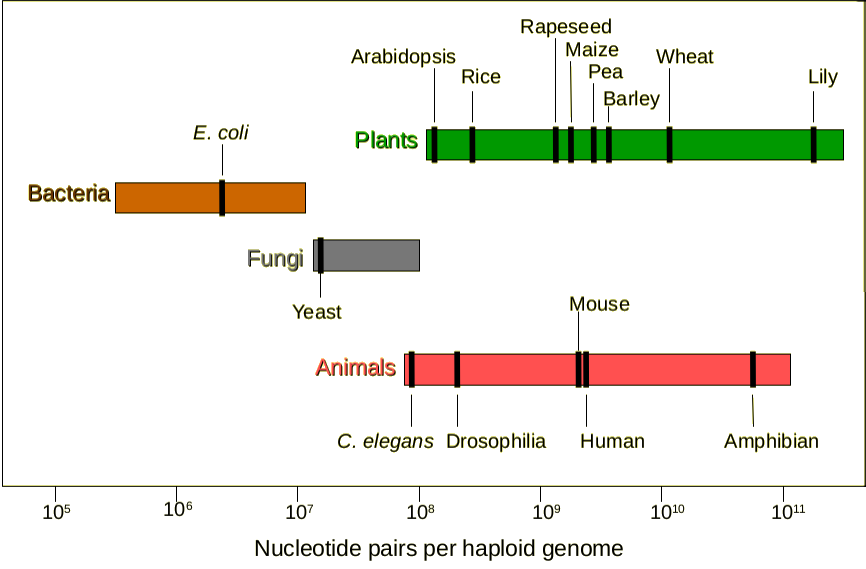
\includegraphics[scale=0.27]{pic_Data/fig1.png}\\
\vspace{0.2cm}
\end{center}
\textbf{Figure 1:} \bsc{Taille relative du génome de plusieurs familles d'organismes}. On remarque nettement que les espèces végétales (plants) possèdent de très grands génomes qui couvrent une fourchette de taille très large ($\approx$ 10$^{8}$ à 10$^{11}$ pb) comparé aux autres groupes. Le blé (wheat), avec son génome estimé à 17 Gb est un génome de très grande taille, même au sein du règne végétal.\\ 
\begin{flushright} 
D'après \textit{Genomes: Organization and Comparisons}, Plant Biotechnology Conference (2009)\\
\end{flushright}
\begin{center}
\rule{10cm}{0.2pt}\\
\vspace{0.7cm}
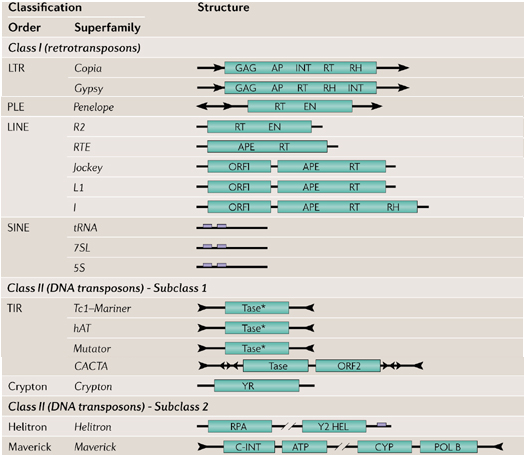
\includegraphics[scale=0.4]{pic_Data/fig2.png}\\
\vspace{0.2cm}
\end{center}
\textbf{Figure 2:} \bsc{Classification simplifiée des éléments transposables}. Celle-ci est basée sur deux classes principales en fonction de la présence (Classe I) ou de l'absence (Classe II) d'un intermédiaire ARN. Chez les céréales, les ET les plus présents sont les rétrotransposons (Classe I), et plus particulièrement les éléments LTR \textit{Copia} et \textit{Gypsy}.

Les rectangles verts représentent les domaines codant des protéines (GAG, protéine de capside ; AP, \textit{protéinase} ; INT, \textit{intégrase} ; RH, \textit{RNAse H} ; RT, \textit{Reverse-Transcriptase} ; Tase, \textit{Transposase} ; ATP, \textit{ATPase}). Celles-ci sont nécessaires aux transpositions des ET dans les génomes.

LTR, long terminal repeat; DIRS, \textit{Dictyostelium} intermadiate repeat sequence; PLE, \textit{Penelope}-like elements; LINE, long interspersed nuclear element; SINE, short interspersed nuclear elements; TIR, terminal inverted repeat.\\
\begin{flushright}
D'après \bsc{Wicker} \textit{et al}., 2007.\\
\end{flushright}
\vfill
\addtocounter{page}{-1}
\newpage

\part{Introduction}
\section{Structure et organisation des génomes végétaux}
La formidable diversité du monde végétal qui nous entoure nous permet d'estimer la grande complexité des génomes végétaux, résultat de plusieurs millions d'années d'évolution et plus récemment de sélection par l'homme. Depuis le décryptage du génome d'\textit{Arabidopsis thaliana} en 2000 (\bsc{The Arabidopsis Genome Initiative}, 2000), les technologies et les débits de séquençage ont beaucoup progressé.

Actuellement, 28 génomes de plantes sont disponibles dans la base de donnée \bsc{PlantGDB} dont notamment, dans la famille des graminées, les génomes du riz, du maïs, du sorgho, de \textit{Brachypodium} et de l'orge, à des degrés de finition variables. L'ancien dogme selon lequel le degré d'évolution d'un individu serait le reflet de la complexité de son génome a été balayé (\bsc{Gregory} \textit{et al.}, 2007). Les génomes végétaux se caractérisent ainsi par une grande diversité de tailles qui dépassent celles observées chez les animaux (Figure 1).

La majorité des séquences qui composent les grands génomes (> 1 Gb) est composée d'éléments génétiques mobiles et répétés, acteurs majeurs de la plasticité et de la capacité d'évolution des organismes. Ces éléments sont appelés éléments transposables lorsqu'ils sont autonomes (codant eux-même les éléments indispensables à leur mobilité au sein du génome) et éléments mobilisables lorsqu'ils n'en sont pas capable.

\section{Les éléments transposables, acteurs majeurs de l'évolution des génomes}
\subsection{Les différentes classes d'éléments transposables}
Ils ont été mis en évidence en 1950 par Barbara MacClintock chez le maïs (\bsc{McClintock}, 1950), c'est à dire avant même la connaissance de la structure de l'ADN. Ces éléments sont uibiquitaires et peuvent représenter de l'ordre de quelques pourcents des séquences chez les petits génomes bactériens (0.5 - 1\% chez \textit{E. coli}, \bsc{Daboussi}, 2006) et jusqu'à 80 - 90\% chez les génomes complexes, comme celui du blé tendre (\bsc{Choulet} \textit{et al.}, 2014). 

La classification des ET eucaryotes, actualisée en 2007, regroupe désormais deux classes principales en fonction de leur mécanisme de transposition, subdivisées en familles et sous-familles comme le montre la figure 2 (\bsc{Wicker} \textit{et al.}, 2007):

% ----------------------------------------
%%% Après page 2
\newpage
\thispagestyle{empty}
\begin{center}
~ \vfill
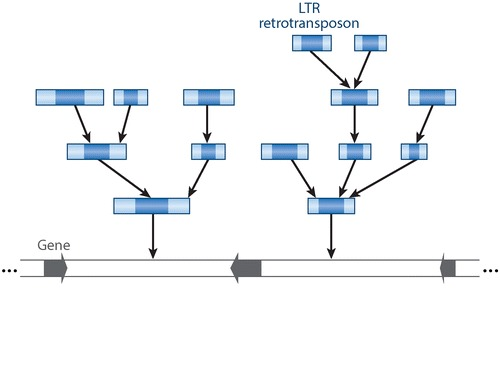
\includegraphics[scale=0.65]{pic_Data/fig3.jpg}\\
\end{center}
\vspace{-1.5cm}
\textbf{Figure 3:} \bsc{Représentation schématique d’événements d'insertion de plusieurs éléments transposables de type LTR dans un génome}. Le modèle pyramidal d'insertion des ET les uns dans les autres permet de reconstruire le profil d'insertion: les ET les plus anciens (insérés en premier dans le génome) sont donc à la base, tandis que les ET au sommet ont été insérés plus récemment à l'intérieur des éléments ayant déjà transposé.
\begin{flushright}
D'après \bsc{Bennetzen} \textit{et al}., 2014.\\
\end{flushright}
\vfill
\addtocounter{page}{-1}
\newpage

\begin{itemize}
\item Classe I: Les ET qui transposent via la transcription d'un ARNm qui est transcrit inversement en ADNc double-brin pouvant s'insérer dans le génome (mécanisme de copier-coller). On appelle ces éléments des rétrotransposons. Les super-familles les plus significativement représentées chez les plantes sont les \textit{Gypsy, Copia}, et \textit{LINE/SINE} (Long/Short Interspersed Nuclear Elements). 
\item Classe II: Les ET qui transposent via leur excision du génome et leur insertion à un nouveau site (mécanisme de couper-coller). Cette classe regroupe également les \textit{Hélitrons} dont le mécanisme de transposition n'est pas encore bien caractérisé mais qui ne semblent pas s'exciser du génome (\bsc{Gupta} \textit{et al.}, 2005). Les super-familles les plus représentées chez les plantes sont les \textit{CACTA, Mutator, Mariner, Harbinger} et \textit{HaT}.
\end{itemize}

\subsection{Impact des éléments transposables sur l'évolution des génomes}
Chez les plantes, c'est principalement les retrotransposons à motifs répétés terminaux (LTR, Long Terminal Repeat) qui sont responsables de la grande taille des génomes (\bsc{Sanmiguel} \textit{et al.}, 1998). Les insertions d'ET actifs dans un génome peuvent se produire n'importe où: dans une région inter-génique, dans un gène, dans un élément régulateur, mais aussi à l'intérieur d'un autre ET inséré plus anciennement selon un modèle pyramidal (Figure 3). La transposition peut donc avoir des effets sur la fonctionnalité des gènes:
\begin{itemize}
 \item L'inactivation du gène par insertion dans sa séquence codante.
 \item La modification de l'expression par insertion de l'ET dans une région régulatrice ou par l'apport de nouvelles séquences régulatrices (\bsc{Goettel} \textit{et al.}, 2010).
 \item La capture de fragments de gènes par un ET ou, dans de rares cas, de gènes entiers (\bsc{Jameson} \textit{et al.}, 2008).
 \item La création de nouveaux gènes par association de portions de gènes différents au sein d'un même ET (\bsc{Jiang} \textit{et al.}, 2004).
\end{itemize}

Les ET ont longtemps été considérés uniquement comme des parasites des génomes et parfois vu comme des éléments égoïstes (\bsc{Orgel} \textit{et al.}, 1980). Toutefois, leur impact sur l'expression des phénotypes est majeur et leur activité de transposition constitue un moteur de l'évolution. Par ailleurs, le projet ENCODE (ENCyclopedia Of DNA Elements), dont le but était de caractériser l'ensemble des éléments intervenant dans l'expression et la régulation de l'expression des gènes chez l'Homme, a mis en lumière l'implication massive des ET dans les mécanismes de régulations. En 2012, le consortium ENCODE a démontré que les gènes proches d'éléments répétés de type \textit{LINE, SINE} ou \textit{LTR}-rétrotransposons (Figure 2) ont une expression plus finement régulée (\bsc{Djebali} \textit{et al.}, 2012). Par ailleurs, beaucoup d'ET sont des sites de fixation de facteurs de transcriptions (\bsc{Wang} \textit{et al.}, 2012) ou sensibles aux DNases (\bsc{Thurman} \textit{et al.}, 2012). Enfin, une liste de 51 traits phénotypiques attribués à des insertions d'ET dans les génomes végétaux a récemment été publiée (\bsc{Vitte} \textit{et al.}, 2014).

% ----------------------------------------
% PB
% ----------------------------------------
\newpage
\thispagestyle{empty}
\null
\addtocounter{page}{-1}
\newpage

\subsection{Développement de marqueurs moléculaires basés sur les éléments transposables}
Les ET ne sont généralement pas soumis à pression de sélection. C'est-à-dire qu'ils ne codent pas de fonctions utiles à l'hôte et les mutations affectant les ET ne sont donc pas contre-sélectionnées. C'est la raison pour laquelle l'évolution moléculaire des ET est plus rapide que l'évolution des gènes (séquences soumises à la sélection naturelle). Les ET sont donc des cibles privilégiées permettant de caractériser les divergences génomiques entre organismes très proches phylogénétiquement, comme différentes variétés au sein d'une espèce. En d'autres termes, de part leur vitesse d'évolution rapide et leur mobilité (leur capacité à générer des réarrangements génomiques) les ET constituent d'excellentes cibles pour identifier des polymorphismes intra-spécifiques. Toutefois, leur nature répétée dans les génomes constitue un frein majeur au développement de marqueurs moléculaires qui doivent être spécifiques d'un locus donné. Ainsi, pour palier à ce problème, il est possible de se focaliser spécifiquement sur les séquences de jonctions entre un ET et son site d'insertion. En effet, la capacité d'insertion aléatoire des ET dans un génome est un atout pour les analyses moléculaires car elle permet de caractériser la présence/absence d'un ET au niveau de son site d'insertion chez différents individus ou différentes variétés. La présence/absence de cet ET peut ainsi être considérée comme les deux formes alléliques d'un même locus et être utilisée pour des analyses de phylogénie ou de diversité.

Différentes techniques ont ainsi été mises au point sur la base de l'amplification PCR des jonctions entre un ET et son site d'insertion. Par exemple, les marqueurs S-SAP (Sequence-Specific Amplified Polymorphism) reposent sur une amplification PCR d'une région située entre une séquence LTR et un site de restriction à proximité (\bsc{Porceddu} \textit{et al.}, 2002). Les marqueurs RBIP (Retrotransposon-Based Insertion Polymorphism) reposent, quant à eux, sur une amplification avec une amorce qui s'hybride dans un retrotransposon et l'autre dans l'ADN flanquant son site d'insertion (\bsc{Flavell} \textit{et al.}, 1998). Enfin, en 2010, \bsc{Paux} \textit{et al}. ont décrit les marqueurs ISBP (Intertion Site-Based Polymorphism) basés sur l'amplification PCR d'un segment d'ADN englobant la jonction (en 5' ou en 3') entre un ET et son site d'insertion (\bsc{Paux} \textit{et al.}, 2010). Le programme \textit{isbpFinder} a ainsi été mis au point dans l'équipe pour identifier ces jonctions dans les séquences du génome du blé et pour développer automatiquement des amorces utilisables en PCR.

Depuis les années 2000 et l'arrivée de ce genre de méthodologies, les publications scientifiques ayant trait aux éléments transposables dans les génomes se multiplient. 

\section{Le blé tendre (\textit{Triticum aestivum L.})}
\subsection{Intérêt agronomique et scientifique de cette espèce}
La production annuelle de 700 millions de tonnes de blé tendre dans le monde (FAO.org) lui donne une importance considérable dans l'alimentation humaine et animale. Le blé est la nourriture de base d'un tiers de la population mondiale et son importance va s'accentuer avec l'accroissement de celle-ci (qui devrait atteindre les 9 milliards d'individus en 2050).

% ----------------------------------------
%%% Après page 4
\newpage
\thispagestyle{empty}
\begin{center}
~ \vfill
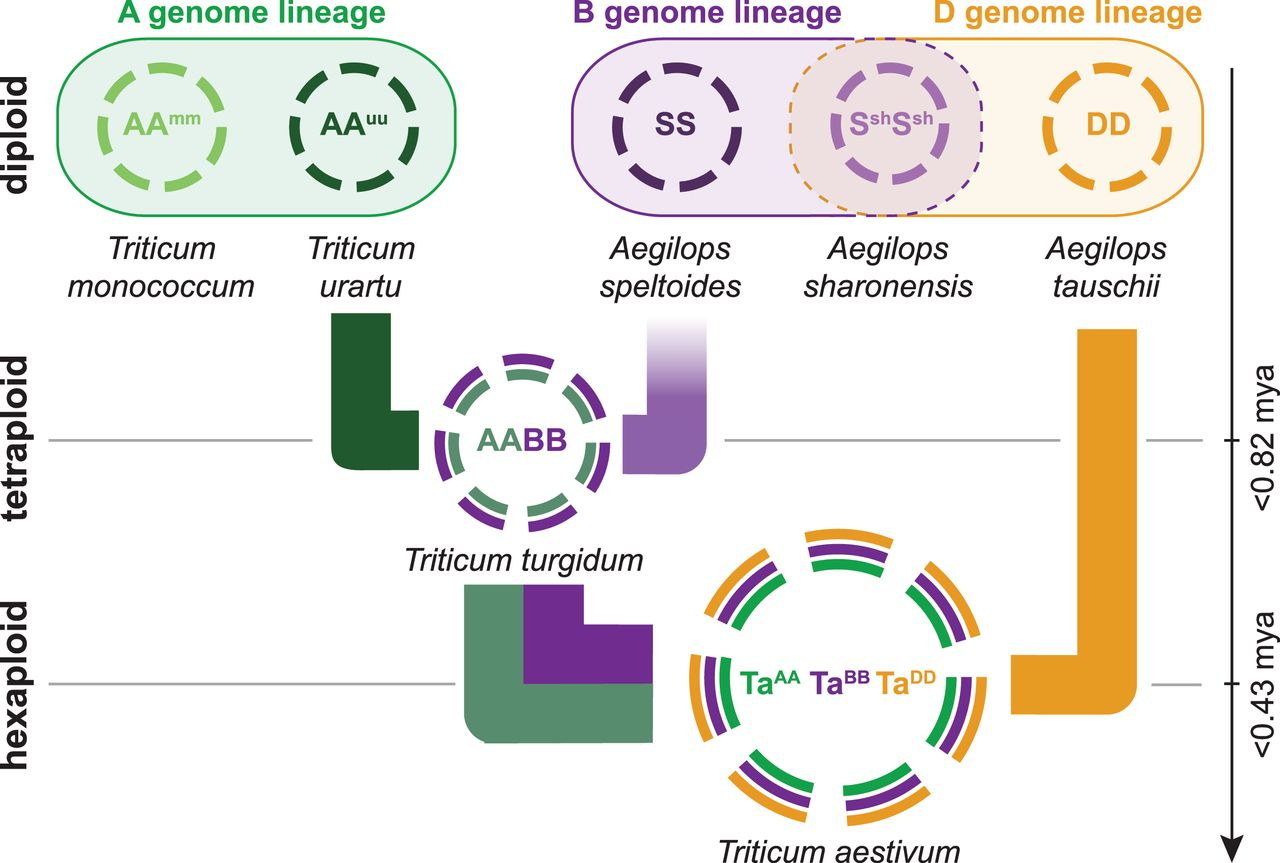
\includegraphics[scale=1.1]{pic_Data/fig5.jpg}\\
\end{center}
\textbf{Figure 4:} \bsc{Représentation schématique de la formation du génome hexaploïde du blé tendre  actuel (\textit{T. aestivum})}. Le premier événement majeur a été un croisement entre deux espèces diploïdes ayant donné naissance, après polyploïdisation à la variété tétraploïde \textit{T. turgidum} (AABB). Un second croisement avec \textit{Ae. tauschii} a apporté le génome D, formant ainsi \textit{T.aestivum} (AABBDD) possédant 7 paires de chromosomes de chacun des 3 génomes.

L'échelle de temps en millions d'années est représentée sur la droite de la figure, datant ainsi les deux évènements majeurs de cette formation.
\begin{flushright}
D'après \bsc{Mayer} \textit{et al.}, 2014\\
\end{flushright}
\vfill
\addtocounter{page}{-1}
\newpage

De plus, une meilleure connaissance du génome du blé sera nécessaire pour répondre aux défis majeurs agronomiques et environnementaux. Cependant, l'évolution des rendements est nulle depuis une quinzaine d'années dans les principaux pays producteurs. Or, cette stagnation n'est pas observée chez d'autres organismes hautement cultivés comme le riz ou le maïs. La principale raison de cette différence est que le génome du blé a longtemps été considéré comme trop complexe, freinant le développement d'outils génomiques performants et la compréhension des caractères phénotypiques de cette espèce.

En effet, le blé tendre possède un génome hexaploïde (AABBDD) provenant de deux évènements de polyploïdisation successifs, comme on peut le voir sur la figure 4 (\bsc{Feldman} \textit{et al.}, 2012):
\begin{itemize}
\item Une première hybridation entre \textit{T. urartu} (AA, 2n=2x=14) et \textit{Ae. speltoides} (BB, 2n=2x=14) a donné naissance au blé tétraploïde (2n=4x=28) il y a environ 0.5 million d'années.
\item Une seconde hybridation de ce tétraploïde avec \textit{Ae. tauschii} (DD, 2n=2x=14) a formé le blé tendre hexaploïde actuel (2n=6x=42) il y a 10 000 ans, au moment de la domestication du blé par l'Homme.
\end{itemize}

La taille de ce génome complet est estimée à environ 17 Gb, soit environ cinq fois le génome humain. Ce caractère réside en partie dans la très forte proportion du génome en séquences répétées, proche de 85\%, soit deux fois plus que l'homme (\bsc{Choulet} \textit{et al.}, 2014). 

Si les deux événements de polyploïdisation sont récents en terme évolutif, les espèces diploïdes (\textit{T. urartu}, \textit{Ae. speltoides} et \textit{Ae. tauschii}) ont divergé d'un ancêtre commun il y a environ 7 millions d'années (\bsc{Marcussen} \textit{et al.}, 2014). Ainsi, le contenu en gènes des sous-génomes A, B et D est encore très conservé (\bsc{Mayer} \textit{et al.}, 2014). Cependant, le contenu en ET est très variable car la plupart de ceux-ci sont éliminés du génome après 3 millions d'années (\bsc{Choulet} \textit{et al.} 2014). Ainsi, les régions intergéniques sont très variables entre les loci homéologues des génomes A, B et D, comme démontré dans l'étude du locus Ha qui contrôle la dureté du grain. (\bsc{Chantret} \textit{et al.}, 2005).

Étudier la génomique du blé possède donc un intérêt double. À la fois fondamental pour la compréhension de la structure, de l'organisation et de l'évolution des génomes complexes, et appliqué étant donné son importance agronomique.

\subsection{Les initiatives de séquençage du génome}
Du fait du poids de cet organisme dans l'alimentation et l'économie mondiale, l'obtention d'une séquence de référence est cruciale. La variété de référence choisie au niveau international est \textit{Chinese Spring}. Un séquençage par approche "shotgun" (séquençage du génome après fragmentation de celui-ci) à faible taux de couverture de cette variété a été réalisée en 2012 sur génome complet (\bsc{Brenchley} \textit{et al.}, 2012). Cette ressource a permis d'identifier environ 96 000 gènes et a servi de base pour l'identification de marqueurs SNP, mais n'a pas permis d'obtenir un assemblage de qualité.

Parallèlement, le consortium IWGSC (International Wheat Genome Sequencing Consortium), fondé en 2005, a entrepris le séquençage du génome via une approche différente. Le développement de la technique de cytométrie de flux a permis la réduction de la complexité du séquençage en passant par le tri des 42 bras de chromosomes (\bsc{Doležel} \textit{et al.}, 2013). L'ADN de chaque bras de chromosome a ainsi été purifié et séquencé par une approche "shotgun", délivrant ainsi la première ébauche de la séquence du génome complet. 

% ----------------------------------------
%%% Après page 5
\newpage
\thispagestyle{empty}
\begin{center}
~ \vfill
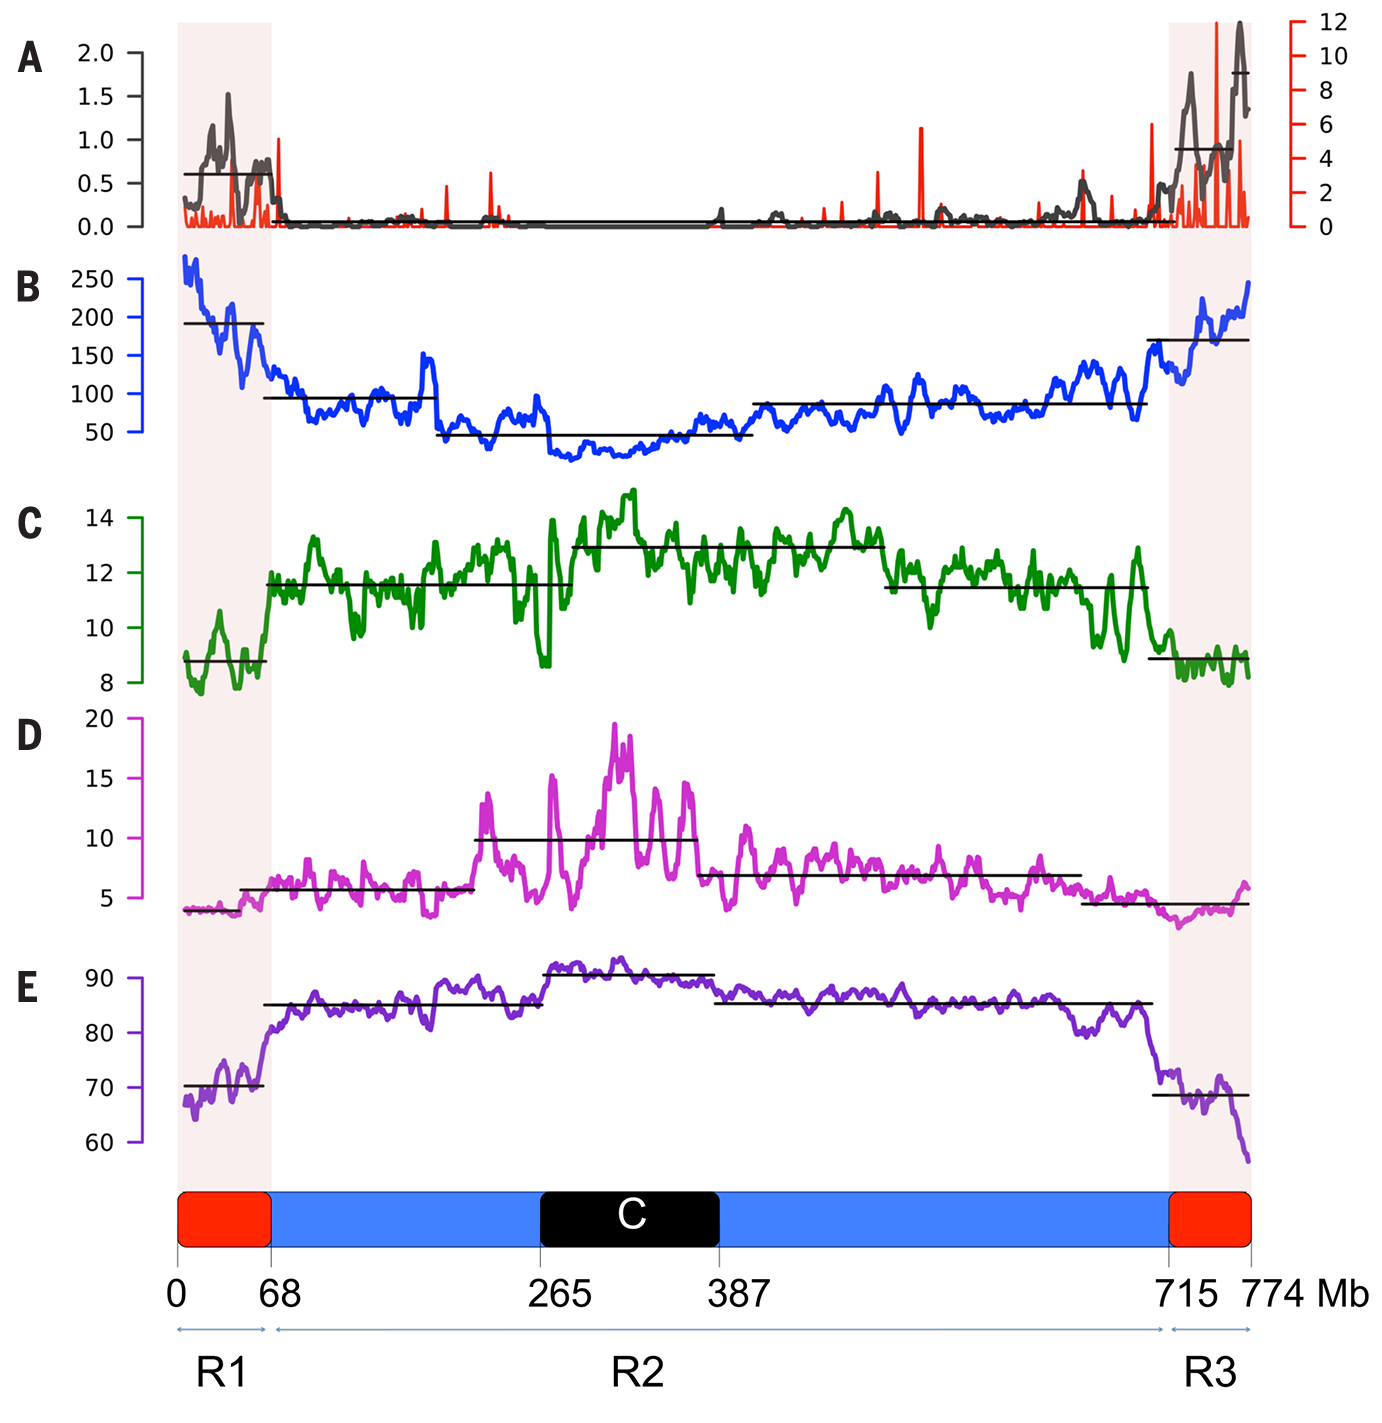
\includegraphics[scale=0.25]{pic_Data/fig_choulet.png}\\
\end{center}
\textbf{Figure 5:} \bsc{Fractionnement du chromosome 3B}. Analyse du taux de recombinaison méiotique (A), de la densité en gène (B), de l'amplitude d'expression de ceux-ci (C), du nombre de transcrits alternatifs par gène (D) et du nombre d'ET (E) le long du chromosome 3B de \textit{Chinese Spring}. La segmentation des valeurs (lignes noires) permet de mettre en évidence 3 régions principales :
\begin{itemize}
\item Une région télomérique R1 (de 0 à 68 Mb).
\item Une région centrale (de 68 à 715 Mb).
\item Une région télomérique R3 (de 715 à 774 Mb).
\end{itemize}
\begin{flushright}
D'après \bsc{Choulet} \textit{et al.}, 2014\\
\end{flushright}
\vfill
\addtocounter{page}{-1}
\newpage

Cette étude a permis d'estimer à 124 000 le nombre de gènes dont 35\% sont portés par le sous-génome B. L'étude de l'expression différentielle des gènes homoéologues au cours du développement de la plante a mis en évidence que la plupart des copies de gènes étaient exprimées, sans dominance particulière d'un sous-génome sur les deux autres (\bsc{Mayer} \textit{et al.}, 2014).

Bien qu'une ébauche de la séquence génomique soit disponible, l'objectif de l'IWGSC est d'obtenir une séquence de référence pour cette espèce. La stratégie qui est suivie pour atteindre cette cible prévoie la construction de cartes physiques (cartes ordonnées provenant de banques BAC contenant des fragments d'ADN génomique) des 21 chromosomes après leur tri en cytométrie. Ainsi, la construction de l'ensemble des cartes physiques devrait s'achever cette année et des projets de séquençage des cartes physiques sont dores et déjà en cours, voire terminés pour 7 chromosomes (www.wheatgenome.org).

\subsection{La séquence de référence du chromosome 3B}
Ce chromosome est le plus grand du génome du blé tendre et est estimé à 886 Mb. Après avoir publié la première carte physique du chromosome 3B en 2008 (\bsc{Paux} \textit{et al.}, 2008), l'équipe a récemment publié la première séquence de référence de ce chromosome (\bsc{Choulet} \textit{et al.}, 2014).

Le résultat de ce travail est un assemblage de 2 808 scaffolds (ensemble de séquences génomiques assemblées et ordonnées) couvrant 833 des 886 Mb totaux estimés du chromosome 3B. L'ancrage de 1 358 scaffolds grâce à 2 594 SNP (Single Nucleotide Polymorphism) ordonnés a permis de construire une pseudomolécule de 774 Mb pour ce chromosome. Une annotation des gènes a été réalisée grâce au pipeline bioinformatique \textit{TriAnnot} (\bsc{Leroy} \textit{et al.}, 2012) et 7 264 gènes codant des protéines ont ainsi pu être identifiés sur la pseudomolécule. Les études d'expression ont permis de déterminer qu'au moins 71\% du contenu en gènes prédit était effectivement transcrit. De plus 3 692 nouveaux loci transcrits codant des ARN non-codant ou des protéines inconnues ont été identifiés.

Un effort particulier a été apporté à la prédiction et l'annotation des éléments transposables le long de cette séquence. Le programme bioinformatique \textit{Clari-TE} a été développé dans l'équipe afin de prédire automatiquement la présence d'ET ainsi que leur mosaïque d'insertion les uns dans les autres (\bsc{Daron} \textit{et al.}, 2014). Ainsi, 252 887 ET (dont 56 233 complets) ont pu être annotés le long du chromosome 3B de \textit{Chinese Spring}, représentant 525 familles au total. Les ET de classe I sont majoritaires sur ce chromosome (67\%, contre 18\% de classe II). De plus, 3 superfamilles représentent à elles seules 80\% des ET totaux : \textit{gypsy}: 47\%, \textit{CACTA}: 16\% et \textit{copia}: 16\%. Ce travail a également permis d'effectuer une datation des évènement d'insertion des ET. Il en ressort que 93\% d'entre eux ont été insérés entre 1 et 3 millions d'années et que ce phénomène est en perte de vitesse depuis le dernier million d'années passé (date de la première polyploïdisation).

L'analyse du taux de recombinaison méotique a également permis de mettre en lumière une compartimentation du chromosome avec des différences marquées entre les régions chromosomiques distales et proximales (Figure 5). En effet, les régions distales (télomériques et subtélomériques), qui correspondent aux régions où se produit très majoritairement la recombinaison méotique, sont plus riches en gènes et plus pauvre en ET que le reste du chromosome. Par ailleurs, ces extrémités chromosomiques sont enrichies en gènes exprimés de façon spécifique (dans peu de conditions), et en fonction liées à l'adaptation de la plante (résistance, réponse aux stress, etc). 

% ----------------------------------------
% PB
% ----------------------------------------
\newpage
\thispagestyle{empty}
\null
\addtocounter{page}{-1}
\newpage

Enfin, ces régions ont accumulé des gènes spécifiques du blé, issus d'événements récents de duplication (\bsc{Rustenholz} \textit{et al.}, 2011). Au contraire, la recombinaison est faible dans la région centrale (péricentromérique) et cette dernière apparaît comme plus stable d'un point de vue évolutif. Elle porte majoritairement des gènes conservés entre les \textit{Paoceae} et exprimés de façon constitutive.

La pseudomolécule du chromosome 3B et l'annotation précise des ET offrent donc une opportunité unique d'étudier le polymorphisme au sein des \textit{Triticeae}. Et notamment le polymorphisme intra-spécifique chez le blé tendre à un niveau de résolution encore jamais atteint chez les génomes complexes.

\section{Objectifs du stage}
L'objectif du stage est de caractériser l'ampleur de la variabilité génomique (le polymorphisme) chez le blé tendre au niveau intra et inter-spécifique (entre variétés hexaploïdes et entre variétés à niveaux de ploïdie différents). L'échelle évolutive considérée dans cette étude est donc très récente. Ainsi, si la recherche de polymorphismes de type SNP (variations alléliques de type substitutions nucléotidiques) permet de caractériser la diversité au niveau des régions géniques, elle ne permet pas d'étudier la variabilité de la partie répétée du génome. Celle-ci, composée d'ET, représente pourtant 85\% du génome complet et constitue la fraction dynamique du génome.

Le paysage transpositionnel chez le blé a été étudié lors de ce stage. Ainsi, il a été possible d'identifier les polymorphismes issus d'insertions/délétions différentielles d'ET entre variétés grâce aux marqueurs ISBP. Ce type de polymorphisme est de type "variations structurales" et plus particulièrement de type présence/absence (PAV, Presence-Absence Variations).

Pour répondre à cette question, la séquence de référence du chromosome 3B représente un outil unique. En effet, la qualité de l'assemblage des séquences a permis d'identifier 252 887 éléments transposables assemblés complètement, et ordonnés le long du chromosome. Par ailleurs, les données de reséquençage du chromosome 3B de 44 variétés de blé (24 tétraploïdes, 20 hexaploïdes), représentant un échantillon homogène au niveau géographique, sont disponibles (Annexe 1). Ces données ont donc été comparées à la séquence de référence de \textit{Chinese Spring}, dont les éléments transposables ont été annotés précédemment, afin d'estimer la variabilité intra et inter-spécifique. 

Ce travail a permis d'établir le paysage transpositionnel du chromosome 3B du blé tendre avec une résolution unique à l'heure actuelle.\\

% ----------------------------------------
% PB
% ----------------------------------------
\newpage
\thispagestyle{empty}
\null
\addtocounter{page}{-1}
\newpage

% ----------------------------------------
% MATÉRIELS ET MÉTHODES
% ----------------------------------------

\part{Matériel et Méthodes}
\textbf{Matériel biologique:} 44 accessions de blés provenant de diverses origines géographiques ont été utilisées pour étudier le paysage transpositionnel au sein du genre \textit{Triticum} (Annexe 1). Ce panel a été sélectionné par le Centre de Ressource Génétique de l'unité GDEC pour présenter un maximum de diversité. En plus de leur origine géographique diverse, 7 espèces sont représentées (\textit{T. carthlicum, T. diccocoides, T. dicoccum, T. durum, T. spelta, T. macha} et \textit{T. aestivum}) ainsi que deux niveaux de ploïdie (24 tétraploïdes et 20 hexaploïdes). Les différents \textit{T. aestivum} sont donc représentatifs de la diversité mondiale du blé tendre, tandis que les autres permettent une analyse phylogénique sur des espèces apparentées. Pour chacune de ces variétés, un tri en cytométrie de flux a été réalisé par l'équipe de J. \bsc{Doležel} (Insitute of Experimental Botany, Olomouc, République Tchèque) afin d'isoler le chromosome 3B.\\

\textbf{Séquences génomiques:} L'ADN trié puis amplifié des chromosomes 3B de chacune des 44 variétés a été séquencé grâce à la technologie Illumina par la société Beckman Coulter Genomics. Brièvement, les chromosomes à séquencer sont découpés en fragments de 300 paires de bases (pb) et déshybridés. Ils sont ensuite amplifiés massivement afin de permettre le séquençage. Celui-ci est effectué grâce à un laser excité lors de l'utilisation, par une ADN polymérase, d'un nucléotide marqué. Chaque fragment d'ADN de 300 pb est ainsi séquencé par les deux bouts, générant deux lectures de 101 pb (séquençage dit "Pair-end"). La couverture (nombre de fois qu'un nucléotide est séquencé) attendue se situait entre 10 et 30x pour chaque variété.\\

\textbf{Extraction des séquences des marqueurs ISBP du chromosome 3B:} Le programme \textit{isbpExtract.pl} a été développé en langage \bsc{perl} durant ce stage afin d'extraire les séquences de jonctions entre les ET et leur site d'insertion (code fourni en annexe 4). Ce programme a permis d'automatiser l'extraction de ces séquences pour l'intégralité des ET prédits le long du chromosome 3B. Cet algorithme réalise les étapes suivantes:
\begin{itemize}
\item Lire la séquence du chromosome 3B.
\item Se connecter à la base de données relationnelle GOW (mySQL) hébergée au laboratoire qui contient l'ensemble des annotations des gènes et ET de la pseudomolecule du chromosome 3B de \textit{Chinese Spring}.
\item Récupérer les positions des ET sur la séquence, c'est-à-dire les positions des jonctions entre les ET et leur site d'insertion.
\end{itemize}
Ensuite, pour chaque position, le programme effectue les actions suivantes:
\begin{itemize}
\item Extraire la séquence comprise entre les nucléotides -75 et +75 autour de chaque jonction.
\item Filtrer les jonctions contenant des "N" dans leur séquence (provenant d'une erreur de séquençage ou d'un trou dans l'assemblage).
\item Éliminer les séquences chevauchantes dans le cas de deux ET proches de moins de 75 pb.
\end{itemize}

% ----------------------------------------
%%% Après page 8
\newpage
\thispagestyle{empty}
\begin{multicols}{2}
\begin{center}
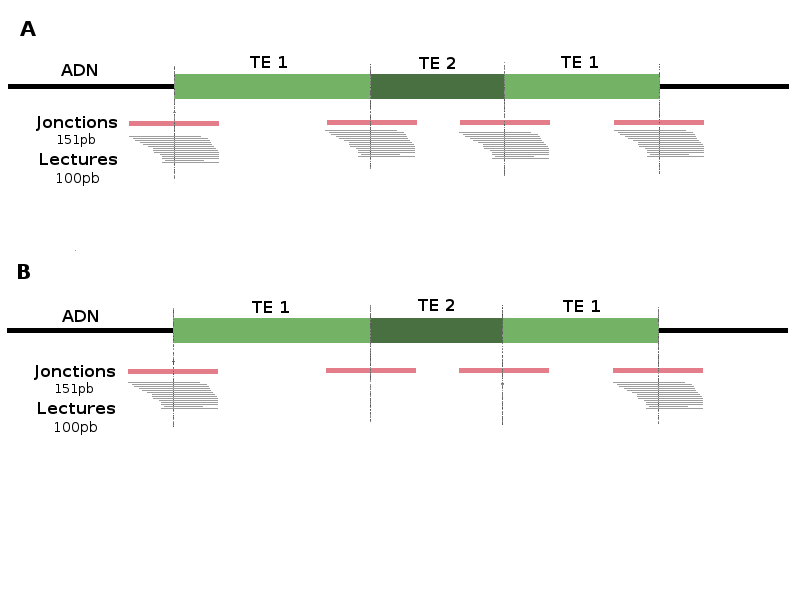
\includegraphics[scale=0.3]{pic_Data/fig4.png}
\vspace{-1.5cm}
\end{center}
\textbf{Figure 6:} \bsc{Représentation schématique de la stratégie utilisée afin de déterminer la présence ou l'absence d'un ET dans une accession}. La séquence génomique contenant les ET 1 et 2 correspond au génome de référence séquencé et annoté. Les marqueurs ISBP (jonctions) sont dessinés à cheval entre les ET et l'ADN à faible nombre de copie ou entre deux ET, puis les lectures de séquençage d'une autre variété sont alignées sur ces marqueurs.

\textbf{A} – Tous les marqueurs sont retrouvées à la même place dans les lectures, les ET sont donc insérés à la même place dans la variété étudiée et dans la référence.

\textbf{B} – Les lectures ne couvrent que la jonction entre TE1 et l'ADN, les jonctions entre TE1 et TE2 ne sont pas retrouvées. L'insertion du TE2 dans le TE1 ne s'est donc pas produite pour cette variété.\\
\end{multicols}
\begin{center}
\rule{10cm}{0.2pt}\\
\vspace{0.5cm}
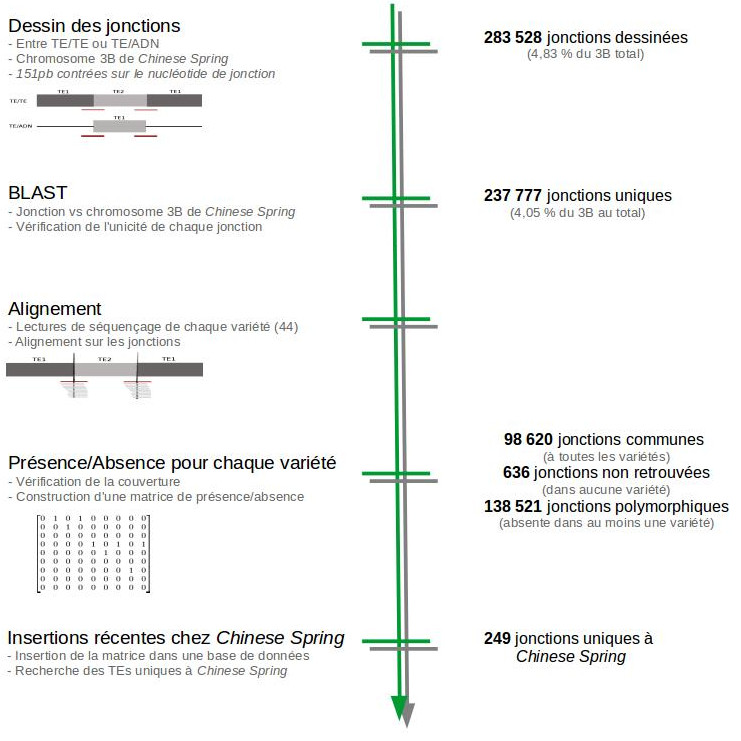
\includegraphics[scale=0.5]{pic_Data/fig6.jpg}\\
\end{center}
\vspace{-0.5cm}
\textbf{Figure 7:} \bsc{Workflow représentant la stratégie globale proposée pour étudier les variations intra-spécifiques dues aux éléments transposables dans les 44 accessions de blé}. Chaque étape est décrite à gauche tandis que les résultats majeurs sont indiqués sur la droite de la flèche.\\
\vfill
\addtocounter{page}{-1}
\newpage

Le programme fournit ainsi un fichier FASTA contenant des séquences de 151 nu. Celles-ci correspondant à des séquences d'ISBP dont la jonction ET/site d'insertion est précisément localisée à la position nucléotidique 76. Une recherche de similarité par BLAST (\bsc{Altschul} \textit{et al.}, 1997) a été réalisée afin d'identifier, et ainsi éliminer, les séquences d'ISBP répétées au sein du chromosome. Seules les séquences extraites uniques présentant 100\% d'identité avec la séquence génomique du chromosome 3B ont été utilisées.\\

\textbf{Alignement des lectures de séquençage sur les séquences des marqueurs ISBP:} Les lectures de séquençage de 101 pb des 44 variétés de blé tendre ont ensuite été alignées avec l'algorithme BWA (\bsc{Li} \textit{et al.}, 2009) sur les séquences des marqueurs ISBP de la variété de référence afin de tester leur présence/absence chez ces lignées. Une tolérance de 4 mésappariements sur 101 pb a été fixée. Le pack d'outil informatique \textit{Samtools} (\bsc{Li} \textit{et al.}, 2009) a été utilisé pour éliminer les duplicats PCR dus au séquençage Illumina. Les alignements ont ensuite été visualisés grâce au logiciel Tablet (\bsc{Milne} \textit{et al.}, 2012). L'ensemble des calculs a été réalisé sur un calculateur haute performance (cluster de calculs, 864 processeurs) hébergé à l'URGI (INRA de Versailles).\\

\textbf{Analyses des données:} Les données expertisées issues des analyses des alignements de séquences ont été intégrées dans une base de données relationnelle mySQL (Annexe 2) et les analyses statistiques et représentations graphiques ont été effectuées avec R (\bsc{R Development Core Team}, 2013) sous environnement Rstudio.\\

% ----------------------------------------
% RÉSULTATS / DISCUSSION
% ----------------------------------------

\part{Résultats / Discussion}
\textbf{Etablissement d'une stratégie \textit{in silico} d'étude du polymorphisme des ET chez les génomes complexes:} Afin d'étudier ces variations de présence/absence au sein des génomes, les données de re-séquençage constituent un excellent outil. Cependant, les ET sont des éléments extrêmement répétés dans les séquences génomiques, parfois à raison de plusieurs dizaines de milliers de copies par chromosome. Ainsi, l'utilisation de logiciels permettant l'alignement de lectures de séquençage pour la détection directe de PAV est inefficace dans ce cas de figure. En effet, les analyses fournissent des résultats inexploitables dus à des alignement multiples pour chaque séquence répétée.

Une nouvelle stratégie a donc été développée ici: l'utilisation de marqueurs ISBP pour la détection de PAV entre variétés. Toutefois, le génotypage par PCR est de faible ou moyen débit, une autre utilisation de ces marqueurs devait donc être mise au point.

Nous pouvons d'ores et déjà prendre pour hypothèse que les données issues du séquençage couvrent uniformément le génome de référence. Ainsi, pour caractériser la présence/absence d'un ET à un locus, il est possible d'utiliser directement ces données afin de les aligner sur les séquences ISBP provenant du génome de \textit{Chinese Spring} (Figure 6 et 7). Le développement de marqueurs de 75 nu de part et d'autre du site d'insertion permet l'alignement de lectures de séquençage de 101 pb qui contiennent obligatoirement cette jonction.

% ----------------------------------------
%%% Après page 9
\newpage
\thispagestyle{empty}
~ \vfill \vspace{-2cm}
\begin{multicols}{2}
\begin{center}
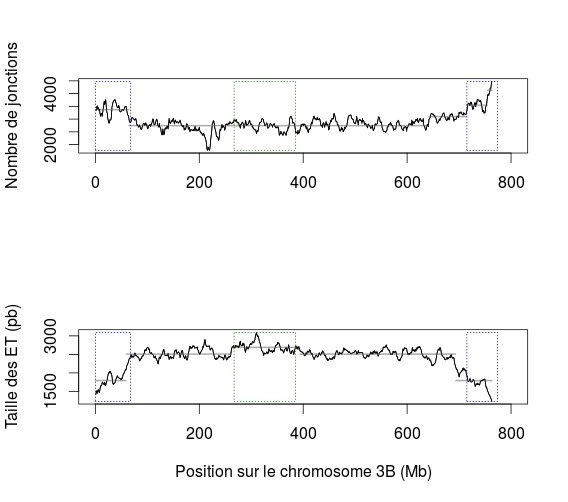
\includegraphics[scale=0.43]{pic_Data/fig7.jpeg}\\
\end{center}
\vspace{-0.3cm}
\textbf{Figure 8:} \bsc{Répartition des 237 777 marqueurs ISBP}. La segmentation de cette distribution des jonctions le long du chromosome 3B montre deux zones aux extrémités ou le nombre de jonctions est plus important (cadres bleus) que dans la zone centrale (cadre vert). 

L'analyse de la taille des ET dans ces différentes zones monte une taille moyenne plus petite dans les régions distales que dans la zone péricentromérique. ~\\

\begin{center}
\vspace{-0.8cm}
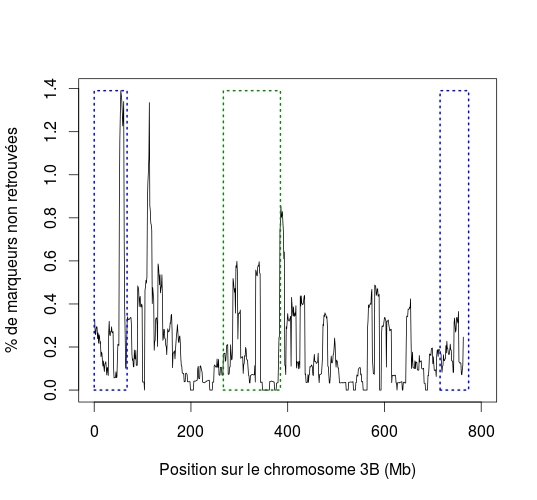
\includegraphics[scale=0.43]{pic_Data/fig8.jpeg}
\end{center}
\textbf{Figure 9:} \bsc{Répartition et proportion des 636 marqueurs dessinés par le programme \textit{isbpExtract} mais non retrouvés lors de leur alignement avec les lectures de séquençage du chromosome 3B de \textit{Chinese Spring}}. On remarque que le pourcentage local de marqueurs non retrouvés par fenêtre de 10 Mb ne dépasse jamais 1,4\% sur la totalité du chromosome.\\ ~\\
\end{multicols}
\vfill
\addtocounter{page}{-1}
\newpage

En effet, l'algorithme BWA aligne les lectures sur les marqueurs ISBP selon un modèle de tout ou rien. Il n'est donc pas possible d'aligner seulement une fraction des 101 pb sur les marqueurs de 151 pb (75+75+1 nu de jonction) sans couvrir le site d'insertion. Ainsi, si une courte lecture issue de NGS s'aligne sur un marqueur ISBP, c'est qu'il est présent dans la variété séquencée. De plus, si les deux jonctions d'un même ET sont présentes dans une accession, c'est que l'insertion de ce dernier est antérieur à la divergence de cette accession avec la variété de référence.\\

\textbf{Extraction des séquences et distribution des ISBP le long du chromosome 3B:} Au total, 252 887 ET ont été prédits le long du chromosome 3B. À partir de ces données d'annotation, le programme \textit{isbpExtract.pl} (Annexe 4) a permis d'extraire 283 528 sous-séquences, correspondant à 151 pb encadrant les jonctions entre ET et leur site d'insertion (marqueurs ISBP). L'élimination des marqueurs répétés le long du chromosome a abouti à la conservation de 237 777 d'entre eux pour les analyses de polymorphisme (Figure 7).

La distribution des marqueurs le long du chromosome a été étudiée dans une fenêtre glissante de 10 Mb se décalant d'un pas de 1 Mb (Figure 8A). On distingue une augmentation significative du nombre de marqueurs dans les régions distales du chromosome. Or il a été démontré que ces régions présentent un pourcentage en ET plus faible que le reste du chromosome (\bsc{Choulet} \textit{et al.}, 2014). Afin d'expliquer cette augmentation, la taille des ET le long du chromosome a été prise en compte (Figure 8B). Leur taille moyenne dans les régions distales est 1.5 fois plus petite que dans la région péricentromérique (respectivement $\begin{simeq}1.7\end{simeq}$ kb et $\begin{simeq}2.5\end{simeq}$ kb). Donc, si les ET représentent une plus faible proportion des séquences, c'est parce qu'ils sont de plus petite taille, mais sont plus nombreux dans les extrémités chromosomiques.

Une chute du nombre de marqueurs ISBP est observée à la position 220 Mb (Figure 8A). Cette région correspond à une insertion d'ADN mitochondrial dans le chromosome 3B, qui est nettement plus pauvre en ET que le génome nucléaire.\\

\textbf{Faisabilité de l'approche et contrôles des données:} La variété \textit{Chinese Spring} a été utilisée comme contrôle positif dans cette analyse, en alignant les lectures de séquençage de cette variété sur les marqueurs dessinés dans son propre génome. Ce contrôle avait pour but d'identifier d'éventuelles erreurs dans la séquence de référence (erreurs d'assemblage créant un ISBP qui n'existe pas en réalité) et/ou d'éventuels biais de séquençage (une région du chromosome n'est pas couverte par le séquençage Illumina du chromosome trié). En effet, l'amplification de l'ADN trié par cytométrie de flux génère obligatoirement des biais. Il est possible, par exemple, que certaines régions du chromosome n'aient pas été amplifiées, donnant lieu à des faux négatifs (ISBP identifiés comme absents alors qu'ils sont présents dans la variété étudiée).

Au total, seulement 636 marqueurs (0,3\%) sur les 237 777 n'ont pas été retrouvés dans l'échantillon de séquences Illumina de la variété de référence. Leur répartition le long du chromosome est homogène (Figure 9), avec un maximum local (par fenêtre de 10 Mb) de faux négatifs égal à 1,4\%. Ces résultats démontrent que les ressources, ainsi que la stratégie mise en place, permettent de répondre précisément à la question posée. Néanmoins, ces 636 marqueurs ISBP ont été éliminés de l'échantillon d'étude.

% ----------------------------------------
% Après page 10
\newpage
\thispagestyle{empty}
~ \vfill
\begin{center}
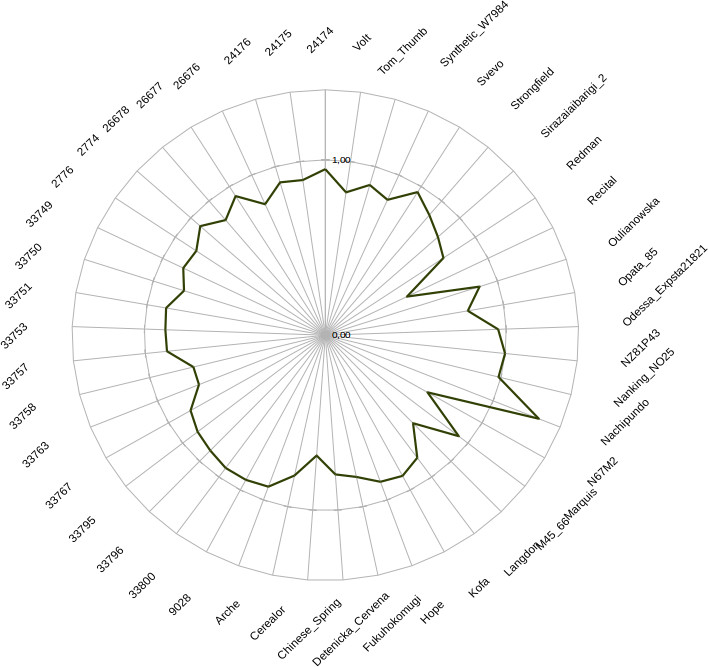
\includegraphics[scale=0.55]{pic_Data/fig9.jpeg}
\end{center}
\textbf{Figure 10:} \bsc{Rapport entre la couverture théorique et la couverture expérimentale}. Celui-ci représente donc la moyenne du nombre de lectures alignées au le nucléotide central de chaque marqueur pour chacune des accessions sur la profondeur de séquençage de l'accession. Ce rapport est $\begin{simeq}1\end{simeq}$ pour toutes les variétés, sauf \textit{Nachipundo} ($\begin{simeq}1.5\end{simeq}$) et \textit{Recital} ($\begin{simeq}0.5\end{simeq}$).
\vfill
\addtocounter{page}{-1}
\newpage

La profondeur du séquençage (rapport entre le nombre de pb issu des lectures de séquençage et le nombre de pb de la région séquencée) est également une paramètre déterminant. Une profondeur trop faible (< 5-6x) pouvant en effet générer beaucoup de faux négatifs. Ainsi, la profondeur du séquençage des 44 variétés a été contrôlée puis comparée à la profondeur théorique attendue. Pour chaque marqueur ISBP, la couverture réelle est mesurée au niveau du nucléotide central de la séquence (nucléotide \No76). Le rapport entre couverture théorique et expérimentale a ainsi permis d'évaluer la qualité du séquençage réalisé pour les 44 variétés (Figure 10).

Cette analyse a permis de montrer que la couverture expérimentale est proche de celle théorique (rapport $\begin{simeq}1\end{simeq}$). Une variété, \textit{Nachipundo}, présente un ratio supérieur à 1. Ceci s'explique par le fait que 14 marqueurs ont une couverture > 10000x (probablement dus au biais d'amplification), valeurs extrêmes qui biaisent la moyenne. A l'inverse, \textit{Recital} présente un ratio $\begin{simeq}0.5\end{simeq}$. Celà suggère que : 
\begin{itemize}
\item Beaucoup des séquences obtenues sont de faible qualité et ne peuvent être alignées.
\item L'échantillon d'ADN issu du tri du chromosome 3B chez cette variété a été contaminé par de l'ADN provenant d'autres chromosomes (contamination habituellement < 5\%).
\end{itemize}
Néanmoins, le taux de couverture observé pour cette accession est de 20x, ce qui est élevé et satisfaisant pour limiter le nombre de faux négatifs.\\

\textbf{Ampleur du polymorphisme et distribution le long du chromosome:} L'approche, par re-séquençage et alignement sur la séquence de référence, utilisée dans cette étude a permis d'identifier les variations structurales (polymorphismes) de type présence/absence: marqueur présent chez \textit{Chinese Spring} et absent chez l'accession comparée. L'inverse n'est pas détectable via cette stratégie. Les polymorphismes observés sont le résultat de deux types d'évènements, soit:
\begin{itemize}
\item D'événements de délétion/excision d'un ET chez l'accession comparée par transposition.
\item D'insertion récente de cet ET chez \textit{Chinese Spring}.
\end{itemize}

Sur les 237 141 marqueurs ISBP utilisables, 138 521 (58\%) ont été identifiés comme polymorphes, c'est-à-dire absents dans au moins une accession. Ceci signifie que plus de la moitié du chromosome 3B n'est pas conservée à l'échelle du genre \textit{Triticeae}. 

Le taux de polymorphisme entre \textit{Chinese Spring} et une accession, est donc représenté ici par un pourcentage de marqueurs non retrouvés. Au sein de l'espèce \textit{T. aestivum}, le polymorphisme atteint en moyenne 15\%. Par ailleurs, le taux de marqueurs non retrouvés varie de 7\% entre \textit{Chinese Spring} et \textit{Sirazaiaibarigi2}, à 45\% entre \textit{Chinese Spring} et \textit{N67M2}.

Les variations locales du taux de polymorphisme ont ensuite été caractérisées dans une fenêtre glissante de 10 Mb le long du chromosome (chaque fenêtre contient en moyenne 3 056 marqueurs) (Annexe 3). Pour chaque accession comparée, le taux de polymorphisme augmente considérablement dans les régions sub-télomériques. En effet, ces régions présentent, pour chaque accession comparée, un taux de polymorphisme 2 à 3 fois plus élevé que la région centrale. Ceci confirme la structuration observée précédemment (\bsc{Choulet} \textit{et al.}, 2014) et démontre, à l'échelle intra-spécifique, que les régions distales évoluent beaucoup plus rapidement que la région centrale. Ceci suggère un lien fort entre intensité de recombinaison et polymorphisme. Le taux de polymorphisme chute dans la région péricentromérique. De plus, cette région stable est encadrée dans les 44 comparaisons par deux pics aux positions 250 et 380 Mb où le polymorphisme est fort.

% ----------------------------------------
% Après page 11
\newpage
\thispagestyle{empty}
\begin{multicols}{2}
\begin{center}
\vspace{-1cm}
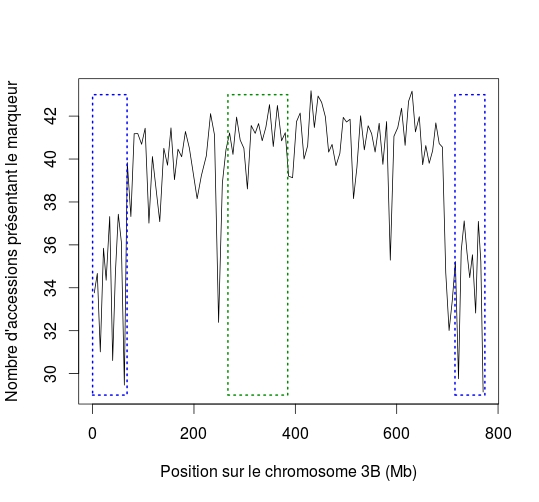
\includegraphics[scale=0.45]{pic_Data/fig10.jpeg}\\
\end{center}
~\\ ~\\ ~\\
\textbf{Figure 11}: \bsc{Nombre de variétés présentant chacun des marqueurs le long du chromosome 3B}. On remarque que les marqueurs ISBP des régions télomériques (cadres bleus) sont retrouvées chez moins de variétés que ceux de la région péricentromérique (cadre vert).\\
\end{multicols}
\vspace{-0.8cm}
\begin{center}
\rule{10cm}{0.2pt}\\
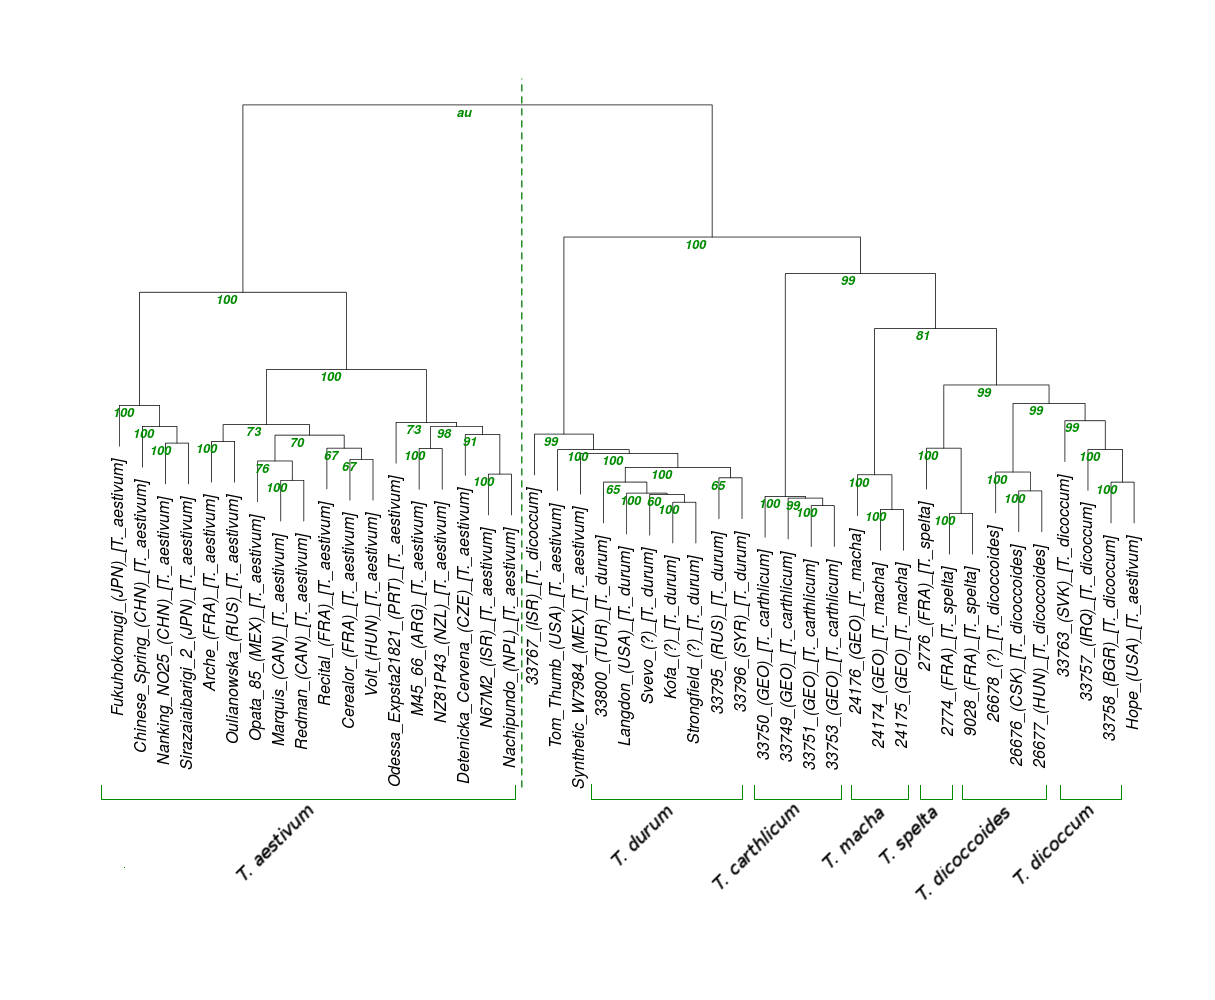
\includegraphics[scale=0.55]{pic_Data/fig11.png}\\
\end{center}
\vspace{-1.5cm}
\textbf{Figure 12}: \bsc{Représentation sous forme d'arbre de la distance entre les 45 variétés de blé étudiées basée sur la matrice de présence/absence de chacun des marqueurs}. L'origine géographique de chaque accession est indiquée entre parenthèse et l'espèce de \textit{Triticum} entre crochets. La ligne verticale sépare les hexaploïdes (à gauche) des tétraploïdes (à droite, sauf \textit{Tom Thumb, Synthetic W7984} et \textit{Hope}), tandis que les nombres indiqués à chaque noeud correspondent au bootstrap 1000 de cet arbre (pourcentage de fois où la branche est représentée telle quelle si le programme génère 1000 fois l'arbre).\\
\vfill
\addtocounter{page}{-1}
\newpage

La figure 11 représente la distribution du niveau de conservation observé parmi les 44 variétés testées. On remarque que les marqueurs portés par la région centrale du chromosome sont conservés chez 41/44 (91\%) accessions en moyenne, alors que ceux situés dans les régions distales sont conservés chez $\begin{simeq}34\end{simeq}$ (77\%) accessions en moyenne. Ces résultats confirment, à une échelle évolutive récente, la grande plasticité des régions terminales et la plus grande conservation de la région centrale.

Cependant, il est aussi possible que cette variabilité soit due à la prédisposition de ces zones à accumuler des SNP au cours du temps. Ce qui pourrait expliquer cette observation. En effet, si ces régions accumulent des mutations à plus haute fréquence, la divergence nucléotidique pourrait avoir empêché l'alignement des séquences entre les variétés testées et les marqueurs de \textit{Chinese Spring}. Les alignements ont effectivement été réalisés en acceptant au maximum 4 mésappariements sur 101 pb au total.\\

\textbf{Analyse phylogénique:} Suite à ces analyses, une matrice de génotypage (présence/absence) des 45 accessions avec les 138 521 marqueurs polymorphes a été générée. Celle-ci a servi de base pour calculer les distances entre accessions et dessiner un arbre phylogénétique (Figure 12). Celui-ci a été construit grâce au package R \textit{pvclust} avec la méthode de clustering \textit{ward} et une distance calculée par méthode de \textit{corrélation}. Sur cet arbre, les différentes espèces testées forment des groupes monophylétiques, avec quelques exceptions. Par ailleurs, les accessions d'origine géographique identique ou proche sont également apparentées sur l'arbre. Ces résultats sont donc cohérents avec la classification antérieure et permettent même de préciser certaines parentés puisque quatre accessions ne sont pas groupées avec les espèces attendues:
\begin{itemize}
\item \textit{Tom Thumb}, qui est hexaploïde (\textit{T. aestivum}), est ici apparenté au groupe \textit{T. durum} (tétraploïde). Ceci peut être expliqué par le fait que cette accession provient d'un croisement dont l'un des parents est une variété de \textit{T. durum} du Tibet.
\item \textit{Hope} est issue d'un croisement entre la variété \textit{Marquis} et un \textit{T. diccocum}, ce qui explique son rapprochement avec le groupe \textit{T. diccocum}.
\item \textit{33767} provient d'un croisement entre un \textit{T. dicoccoides} et un \textit{T. durum}, d'où sa proche parenté avec le groupe des \textit{T. durum}.
\item \textit{Synthetic W7984} est un blé synthétique obtenu par hydridation entre \textit{T. urartu} et \textit{Ae. speltoides}, ce qui explique la parenté de son génome B avec celui du groupe des \textit{T. durum}.
\end{itemize}

La séparation entre hexaploïdes et tétraploïdes est également bien retrouvée sur cet arbre (sauf pour l'accession \textit{Hope}, voir ci-dessus). La variabilité intra-spécifique due aux ET permet donc bien de discriminer les différentes accessions en fonction de leur niveau de ploïdie, de leur origine géographique mais aussi suivant la variété étudiée de \textit{Triticum}. Un tel niveau de résolution (138 521 marqueurs) n'avait encore jamais été atteint. Il permettrait d'établir une phylogénie très précise du genre \textit{Triticum} complet. Il est même possible de retrouver le pédigrée d'une variété en particulier, comme ce fut le cas pour les 4 accessions dont le positionnement dans l'arbre ne correspondait pas à celui attendu au regard de la classification antérieure.\\

\textbf{Intensité de la transposition chez le blé:} La stratégie mise en place permet également de caractériser le taux de transposition des ET dans le génome à une échelle évolutive très récente. En effet, 249 marqueurs dérivés d'ET n'ont été retrouvés que chez \textit{Chinese Spring}. 

% ----------------------------------------
% Après page 12
\newpage
\thispagestyle{empty}
~ \vfill
\begin{multicols}{3}
\begin{center}
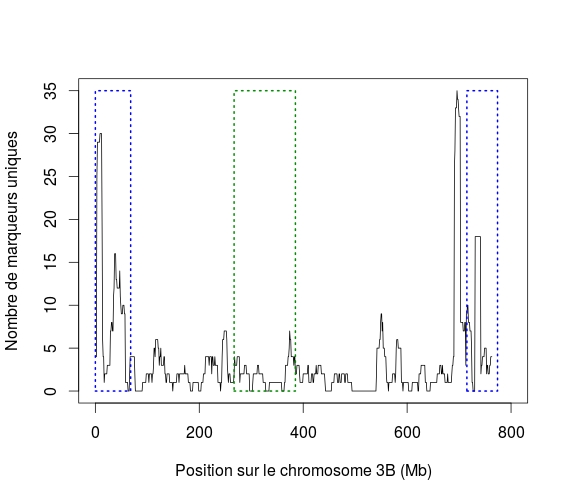
\includegraphics[scale=0.3]{pic_Data/fig12.jpeg}\\
\end{center}
\textbf{Figure 13}: \bsc{Répartition le long du chromosome 3B des marqueurs retrouvés uniquement chez la variété \textit{Chinese Spring}}. Ceux-ci représentent donc des insertions d'ET très récentes. On retrouve beaucoup plus d'éléments nouvellement insérés aux extrémités télomériques (cadres bleus) que dans la zone péricentromérique (cadre vert).\\ ~\\ ~\\ ~\\ ~\\ ~\\ ~\\

\begin{center}
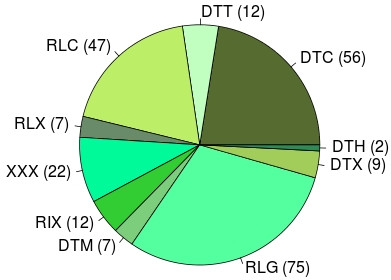
\includegraphics[scale=0.4]{pic_Data/fig13.jpeg}\\
\end{center}
\textbf{Figure 14}: \bsc{Répartition des ET nouvellement insérés chez \textit{Chinese Spring} en fonction de leur famille}. On note la présence de 86 transposons à ADN: DTC (\textit{CACTA}), DTT (\textit{Mariner}), DTH (\textit{Harbinger}), DTX (TIR non identifié), DTM (\textit{Mutator}) et 141 rétrotransposons: RLC (\textit{Copia}), RLG (\textit{Gypsy}), RIX (LINE non identifié), RLX (LTR non identifié). 22 ET n'avaient pas de famille correspondante dans la base de donnée (XXX).

\begin{center}
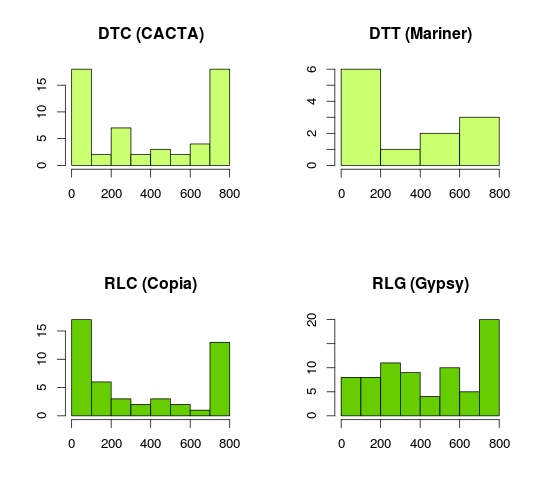
\includegraphics[scale=0.33]{pic_Data/fig14.jpeg}
\end{center}
\textbf{Figure 15}: \bsc{Distribution le long du Chromosome 3B de \textit{Chinese Spring} du nombre d'insertions récentes d'éléments transposable des 4 familles principales}. L'activité des ET semble plus forte aux extrémités télomériques que ce soit pour les transposons à ADN (vert pâle) ou pour les rétrotransposons (vert foncé).\\ ~\\ ~\\ ~\\ ~\\
\end{multicols}
\vfill
\addtocounter{page}{-1}
\newpage

Ceux-ci représentent donc des insertions très récentes d'ET dans le génome de cette accession, après sa divergence avec la variété la plus proche. Ceci indique que les ET ne sont pas totalement éteints mais qu'une activité de transposition existe. Bien que des événements d'insertion aient touché toutes les régions chromosomiques, ils ont principalement eu lieu aux extrémités télomériques (Figure 13). Ce résultat suggère qu'il existe bien une insertion préférentielle des ET dans les régions recombinogènes. Les types d'ET qui sont encore actifs ont ensuite pu être étudiés.

Une plus forte proportion de rétrotransposons (141 insertions, 57\%) que de transposons de classe II (86 insertions, 35\%) a été observée (Figure 14), reflétant l'abondance des retrotransposons dans le génome et plus particulièrement les \textit{Copia} (RLC) et \textit{Gypsy} (RLG). Ici, ces deux types d'ET représentent à eux deux 49\% des insertions récentes d'ET chez \textit{Chinese Spring}. Les \textit{CACTA} (DTC) sont les transposons de classe II les plus abondants chez le blé, et ils représentent 56 (22\%) événements d'insertion récents chez \textit{Chinese Spring}. Ces résultats vont à l'encontre des premières hypothèses émises précédemment sur la dynamique des ET qui suggéraient que seules quelques familles sont actives au sein du génome à une période précise. Les autres étant éteintes, notamment par la machinerie de "silencing". Ces nouvelles données permettent donc une remise en cause des modèles d'évolution du génome. Ils sont ainsi d'un grand intérêt pour mieux comprendre les forces évolutives à l'oeuvre chez les génomes complexes.

La distribution des événements d'insertion le long du chromosome a été calculée pour les 4 superfamilles d'ET les plus représentées ici : \textit{CACTA} (DTC), \textit{Mariner} (DTT), \textit{Gypsy} (RLG), \textit{Copia} (RLC) (Figure 15). Elles présentent toutes une insertion préférentielle dans les régions terminales. On remarque que les \textit{CACTA}, les \textit{Mariner} et les \textit{Copia} ont une activité plus forte sur le bras court (de 0 à 300 Mb) que sur le bras long.\\

\textbf{Capture de gènes:} Des travaux antérieurs sur le chromosome 3B avaient permis d'identifier des événements de capture de gènes par des ET. Nous avons initié un travail dans le but de croiser les données de polymorphisme avec ces informations de capture de gènes. Ceci avait pour objectif de dater, sur la base de l'arbre phylogénétique, ces évènements de capture. Un \textit{CACTA} (appelé \bsc{93\_v443\_1826} dans l'annotation des ET) ayant capturé le gène \bsc{traes3bf182600010cfd\_t1} codant une protéine de type VAMP-like putative (Vesicule-Associated Membrane Protein) est apparu comme un bon candidat pour cette analyse. D'après les résultats de polymorphisme, ce \textit{CACTA} est conservé entre les 4 variétés asiatiques apparentées sur l'arbre (\textit{Chinese Spring, Fukuhokomugi, Nanking \No 25} et \textit{Sirazaiaibarigi 2}) et totalement absent de toutes les autres accessions. Ceci indique que l'événement de capture de gène s'est produit spécifiquement dans la lignée des blés asiatiques avant leur divergence.

Grâce à la stratégie mise en place au cours de ce stage, il est maintenant possible de dater les évènements de capture de gènes et les transpositions récentes.\\

% ----------------------------------------
% PB
% ----------------------------------------
\newpage
\thispagestyle{empty}
\null
\addtocounter{page}{-1}
\newpage

% ----------------------------------------
% CONCLUSIONS / PERSPECTIVES
% ----------------------------------------

\part{Conclusions / Perspectives}
Lors de ce stage, le polymorphisme intra et inter-spécifique du groupe des \textit{Triticeae} a été étudié à un très fort niveau de résolution à l'aide de la séquence du chromosome 3B et de données de re-séquençage générées chez 44 accessions hexaploïdes et tetraploïdes maximisant la diversité mondiale. En effet, 138 521 marqueurs polymorphes dérivés d'ET ont été identifiés au cours de cette étude. Ceux-ci représentent 58\% des ET du chromosome 3B qui sont polymorphes (présence/absence) dans notre échantillon. Deux régions de forte variabilité localisées aux extrémités chromosomiques, et une région plus conservée autour du centromère, ont ainsi pu être mises en évidence.

Cette méthode a permis de générer une matrice de distances entre les accessions et donc de dresser un dendrogramme. Celui-ci a confirmé l'apparentement attendu sur la base de la classification antérieure (au niveau de l'espèce), de l'origine géographique des accessions, et de leur niveau de ploïdie. Il est également possible de confirmer le pedigree d'une accession, en particulier si celui-ci est mal connu.

Le paysage transpositionnel récent du chromosome 3B de \textit{Chinese Spring} a également pu être étudié. Les régions télomériques ont été définies comme les zones d'insertion préférentielles des ET de classe I et II. Par ailleurs, 9 superfamilles sont actives et ont transposé très récemment dans le génome de \textit{Chinese Spring}.

En terme de perspectives, d'un point de vue méthodologique, les résultats présentés ici pourraient être comparés à ceux obtenus avec des logiciels "clé en main" permettant d'identifier les variations structurales de type présence/absence (PAV) à partir de données de ré-séquençage (\textit{e.g.} SSAHA2, Sanger Institute). Par ailleurs, une validation par PCR pourrait également être entreprise afin de valider les résultats obtenus \textit{In Silico} afin de déterminer la sensibilité de la méthode développée ici. L'analyse pourrait également être effectuée en réduisant petit à petit le nombre de marqueurs utilisés. Ceci afin de déterminer le nombre minimum de marqueurs ISBP nécessaires, parmi les 138 521 polymorphiques, pour générer un arbre tel que celui présenté dans cette étude.

L'étude plus fine des différences entre hexaploïdes et tétraploïdes pourrait être effectuée, notamment pour mettre en évidence les polymorphismes qui sont dus à l'hexaploïdisation. En effet, de nombreuses études ont montré que les événements de polyploïdisation étaient souvent accompagnés d'une réactivation des ET, et donc d'un bouleversement génomique. L'approche développée ici permettra de confirmer ou non ces hypothèses.

Enfin, les polymorphismes identifiés ici pourront être corrélés à des différences phénotypiques entre accessions via des approches de génétique d'association. Ceci permettra peut-être d'identifier des gènes, ou des ET régulateurs de gènes contrôlant des caractères agronomiques d'intérêt.\\

% ----------------------------------------
% PB
% ----------------------------------------
\newpage
\thispagestyle{empty}
\null
\addtocounter{page}{-1}
\newpage

% ----------------------------------------
% REFLEXION PERSONNELLE
% ----------------------------------------

\part{Réflexion personnelle}
Mon opinion vis-à-vis de ce stage est très positive. En effet, je trouve que le stage en laboratoire de recherche est une formidable opportunité de mettre en pratique les connaissances théoriques acquises. Une expérience professionnelle de 5 mois et demi, comme j'ai eu la chance de pouvoir effectuer, permet de mieux comprendre la finalité des notions acquises à l'université, mise en perspective qu'il est souvent difficile d'appréhender pendant les cours. C'est ce genre d'expériences qui est également susceptible de nous donner des indices sur la façon dont notre avenir scientifique sera construit.

Lors du stage, discuter avec des personnes travaillant sur un même organisme, mais avec des thématiques différentes, m'a permis de faire le lien entre plusieurs matières scientifiques. Il est également plaisant de pouvoir se focaliser sur une question biologique et un sujet précis durant plusieurs mois. Cela permet de pouvoir s'investir davantage.

Ce sujet de stage était de plus intéressant au regard des compétences qu'il m'a permis d'acquérir. La bioinformatique est un outil nouveau pour moi que j'ai pu découvrir et commencer à maîtriser. Je me suis rendu compte que contrairement aux idées reçues, ce domaine est accessible pour des biologistes sans formation préalable particulière. Grâce aux membres de l'équipe SEVEN et à leurs nombreux conseils, j'ai donc pu appréhender un outil extrêmement puissant permettant de traiter un éventail très large de données biologiques ne se limitant pas aux séquences génomiques du blé tendre. En effet, l'avancée très rapide des technologies provoque à l'heure actuelle une hausse considérable de la quantité de données à analyser, d'où l'intérêt de la bioinformatique pour pouvoir les traiter.

Étudier une espèce telle que le blé, qui est un organisme d'importance mondiale, a également été une source de motivation pour moi. Le travail sur les éléments transposables reste un domaine assez méconnu dans la biologie, bien qu'ils occupent une place prépondérante dans les génomes. Explorer un tel sujet m'a beaucoup plu, et me plaira encore au vu des analyses restant à effectuer sur ces éléments, rien que chez le blé tendre.

Enfin, la rédaction d'un rapport est pour moi un très bon exercice de réflexion et de prise de recul sur le travail accompli. Cela m'a également permis d'acquérir des connaissances dans le domaine de la génomique des plantes grâce à la recherche et la synthèse bibliographique ainsi que dans l'édition de documents scientifiques grâce à l'utilisation du langage de composition de documents \LaTeX.

% ----------------------------------------
% PB
% ----------------------------------------
\newpage
\thispagestyle{empty}
\null

% ----------------------------------------
% BIBLIOGRAPHIE
% ----------------------------------------

\newpage
\pagestyle{empty}
\tocless\part{Bibliographie}
\begin{flushleft}

\textbf{Altschul S.F., Madden T.L., Schäffer A.A., Zhang J., Zhang Z., Miller W., Lipman D.J.} (1997). Gc. \textit{Nucleic Acids Res}. \textbf{17}:3389–3402.\\
\vspace{0.3cm}
\textbf{Brenchley R., Spannagl M., Pfeifer M., Barker G.L.A., D’Amore R., Allen A.M., McKenzie N., Kramer M., Kerhornou A., Bolser D., et al.} (2012). Analysis of the bread wheat genome using whole-genome shotgun sequencing. \textit{Nature}. \textbf{491}:705–710.\\
\vspace{0.3cm}
\textbf{Chantret N., Salse J., Sabot F., Rahman S., Bellec A., Laubin B., Dubois I., Dossat C., Sourdille P., Joudrier P., et al.} (2005). Molecular Basis of Evolutionary Events That Shaped the Hardness Locus in Diploid and Polyploid Wheat Species (Triticum and Aegilops). \textit{Plant Cell}. \textbf{17}:1033–1045.\\
\vspace{0.3cm}
\textbf{Choulet F., Alberti A., Theil S., Glover N., Barbe V., Daron J., Pingault L., Sourdille P., Couloux A., Paux E., et al.} (2014). Structural and functional partitioning of bread wheat chromosome 3B. \textit{Science}. \textbf{345}.\\
\vspace{0.3cm}
\textbf{Daboussi M.J.} (2006). The repetitive DNA content of genomes. \textit{Formation INRA}.\\
\vspace{0.3cm}
\textbf{Djebali S., Davis C.A., Merkel A., Dobin A., Lassmann T., Mortazavi A., Tanzer A., Lagarde J., Lin W., Schlesinger F., et al.} (2012). Landscape of transcription in human cells. \textit{Nature}. \textbf{489}:101–108.\\
\vspace{0.3cm}
\textbf{Daron J., Glover N., Pingault L., Theil S., Jamilloux V., Paux E., Barbe V., Mangenot S., Alberti A., et al.} (2014). Organization and Evolution of Transposable Elements along the Wheat Chromosome 3B. \textit{Under submission}.\\
\vspace{0.3cm}
\textbf{Doležel J., Vrána J., Cápal P., Kubaláková M., Burešová V., Šimková H.} (2013). Advances in plant chromosome genomics. \textit{Biotechnology Advances}. \textbf{32}:122-136.\\
\vspace{0.3cm}
\textbf{Feldman M., and Levy A.A.} (2012). Genome Evolution Due to Allopolyploidization in Wheat. \textit{Genetics}. \textbf{192}:763–774.\\
\vspace{0.3cm}
\textbf{Flavell A.J., Knox M.R., Pearce S.R., Ellis T.H.} (1998). Retrotransposon-based insertion polymorphisms (RBIP) for high throughput marker analysis. \textit{Plant J.}. \textbf{16}:643–650.\\
\vspace{0.3cm}
\textbf{Gregory T.R., Nicol J., Tamm H., Kullman B., Kullman K., Leitch I.J., Murray B., Kapraun D., Greilhuber J., et al.} (2007). Eukaryotic genome size databases. \textit{Nucleic Acide Res}. \textbf{35}:332-338.\\
\vspace{0.3cm}
\textbf{Goettel W., and Messing J.} (2010). Divergence of gene regulation through chromosomal rearrangements. \textit{BMC Genomics}. \textbf{11}:678-682.\\
\vspace{0.3cm}
\textbf{Gupta S., Gallavotti A., Stryker G.A., Schmidt R.J., and Lal S.K.} (2005). A novel class of Helitron- related transposable elements in maize contain portions of multiple pseudogenes. \textit{Plant Mol Biol}. \textbf{57}:115–127.\\
\vspace{0.3cm}
\textbf{Jameson N., Georgelis N., Fouladbash E., Martens S., Hannah L.C., and Lal S.} (2008). Helitron mediated amplification of cytochrome P450 monooxygenase gene in maize. \textit{Plant Mol Biol}. \textbf{67}:295–304.\\
\vspace{0.3cm}
\textbf{Jiang N., Bao Z., Zhang X., Eddy S.R., and Wessler S.R.} (2004). Pack-MULE transposable elements mediate gene evolution in plants. \textit{Nature}. \textbf{431}:569–573.\\
\vspace{0.3cm}
\textbf{Leroy P., Guilhot N., Sakai H., Bernard A., Choulet F., Theil S., Reboux S., Amano N., Flutre T., Pelegrin C., et al.} (2012). TriAnnot: A Versatile and High Performance Pipeline for the Automated Annotation of Plant Genomes. \textit{Front Plant Sci}. \textbf{3}.\\
\vspace{0.3cm}
\textbf{Li H., and Durbin R.} (2009). Fast and accurate short read alignment with Burrows-Wheeler transform. \textit{Bioinformatics}. \textbf{25}:1754–1760.\\
\vspace{0.3cm}
\textbf{Li H., Handsaker B., Wysoker A., Fennell T., Ruan J., Homer N., Marth G., Abecasis G., Durbin R.} (2009). The Sequence Alignment/Map format and SAMtools. \textit{Bioinformatics}. \textbf{25}:2078–2079.\\
\vspace{0.3cm}
\textbf{Marcussen T., Sandve S.R., Heier L., Spannagl M., Pfeifer M., Jakobsen K.S., Wulff B.B., Steuernagel S., Mayer K.F., et al.} (2014). Ancient hybridizations among the ancestral genomes of bread wheat. \textit{Science}. \textbf{345}.\\
\vspace{0.3cm}
\textbf{Mayer K.F.X., Rogers J., Dolezel J., Pozniak C., Eversole K., Feuillet C., Gill B., Friebe B., Lukaszewski A.J., Sourdille P., et al.} (2014). A chromosome-based draft sequence of the hexaploid bread wheat (Triticum aestivum) genome. \textit{Science}. \textbf{345}.\\
\vspace{0.3cm}
\textbf{McClintock B.} (1950). The origin and behavior of mutable loci in maize. \textit{Proc. Natl. Acad. Sci. U.S.A.} \textbf{36}:344–355.\\
\vspace{0.3cm}
\textbf{Milne I., Stephen G., Bayer M., Cock P.J.A., Pritchard L., Cardle L., Shaw P.D., and Marshall D.} (2013). Using Tablet for visual exploration of second-generation sequencing data. \textit{Brief. Bioinformatics}. \textbf{14}:193–202.\\
\vspace{0.3cm}
\textbf{Orgel L.E., and Crick F.H.} (1980). Selfish DNA: the ultimate parasite. \textit{Nature}. \textbf{284}:604–607.\\
\vspace{0.3cm}
\textbf{Paux E., Sourdille P., Salse J., Saintenac C., Choulet F., Leroy P., Korol A., Michalak M., Kianian S., Spielmeyer W., et al.} (2008). A physical map of the 1-gigabase bread wheat chromosome 3B. \textit{Science}. \textbf{322}:101–104.\\
\vspace{0.3cm}
\textbf{Paux E., Sourdille P., Mackay I., Feuillet C.} (2012). Sequence-based marker development in wheat: Advances and applications to breeding. \textit{Biotechnology Advances}. \textbf{30}:1071–1088.\\
\vspace{0.3cm}
\textbf{Porceddu A., Albertini E., Barcaccia G., Marconi G. et al.} (2002). Development of S-SAP markers based on an LTR-like sequence from Medicago sativa L. \textit{Mol Genet Genomics}. \textbf{267}:107–114.\\
\vspace{0.3cm}
\textbf{R Development Core Team} (2013). R: A language and environment for statistical computing.\\
\vspace{0.3cm}
\textbf{Rustenholz C., Choulet F., Laugier C., Safar J., Simkova H., Dolezel J., Magni F., Scalabrin S., Cattonaro F., Vautrin S., et al.} (2011). A 3,000-loci transcription map of chromosome 3B unravels the structural and functional features of gene islands in hexaploid wheat. \textit{Plant Physiol}. \textbf{157}:1596–1608.\\
\vspace{0.3cm}
\textbf{Sanmiguel P., and Bennetzen J.L.} (1998). Evidence that a Recent Increase in Maize Genome Size was Caused by the Massive Amplification of Intergene Retrotransposons. \textit{Ann Bot}. \textbf{82}:37–44.\\
\vspace{0.3cm}
\textbf{The Arabidopsis Genome Initiative} (2000). Analysis of the genome sequence of the flowering plant Arabidopsis thaliana. \textit{Nature}. \textbf{408}:796–815.\\
\vspace{0.3cm}
\textbf{Thurman R.E., Rynes E., Humbert R., Vierstra J., Maurano M.T., Haugen E., Sheffield N.C., Stergachis A.B., Wang H., Vernot B., et al.} (2012). The accessible chromatin landscape of the human genome. \textit{Nature}. \textbf{489}:75–82.\\
\vspace{0.3cm}
\textbf{Vitte C., Fustier M.-A., Alix K., and Tenaillon M.I.} (2014). The bright side of transposons in crop evolution. \textit{Brief Funct Genomics}. \textbf{13}:276-295.\\
\vspace{0.3cm}
\textbf{Wang J., Zhuang J., Iyer S., Lin X., Whitfield T.W., Greven M.C., Pierce B.G., Dong X., Kundaje A., Cheng Y., et al.} (2012). Sequence features and chromatin structure around the genomic regions bound by 119 human transcription factors. \textit{Genome Res}. \textbf{22}:1798–1812.\\
\vspace{0.3cm}
\textbf{Wicker T., Sabot F., Hua-Van A., Bennetzen J.L., Capy P., Chalhoub B., Flavell A., Leroy P., Morgante M., Panaud O., et al.} (2007). A unified classification system for eukaryotic transposable elements. \textit{Nat. Rev. Genet}. \textbf{8}:973–982.
\end{flushleft}

% ----------------------------------------
% PB
% ----------------------------------------
\newpage
\thispagestyle{empty}
\null

% ----------------------------------------
% ANNEXES
% ----------------------------------------

\newpage
\pagestyle{empty}
~ \vfill \vspace{-1cm}
\tocless\part{Annexes}
\vfill

\newpage
\begin{center}
\Large\textbf{Annexe 1}\\
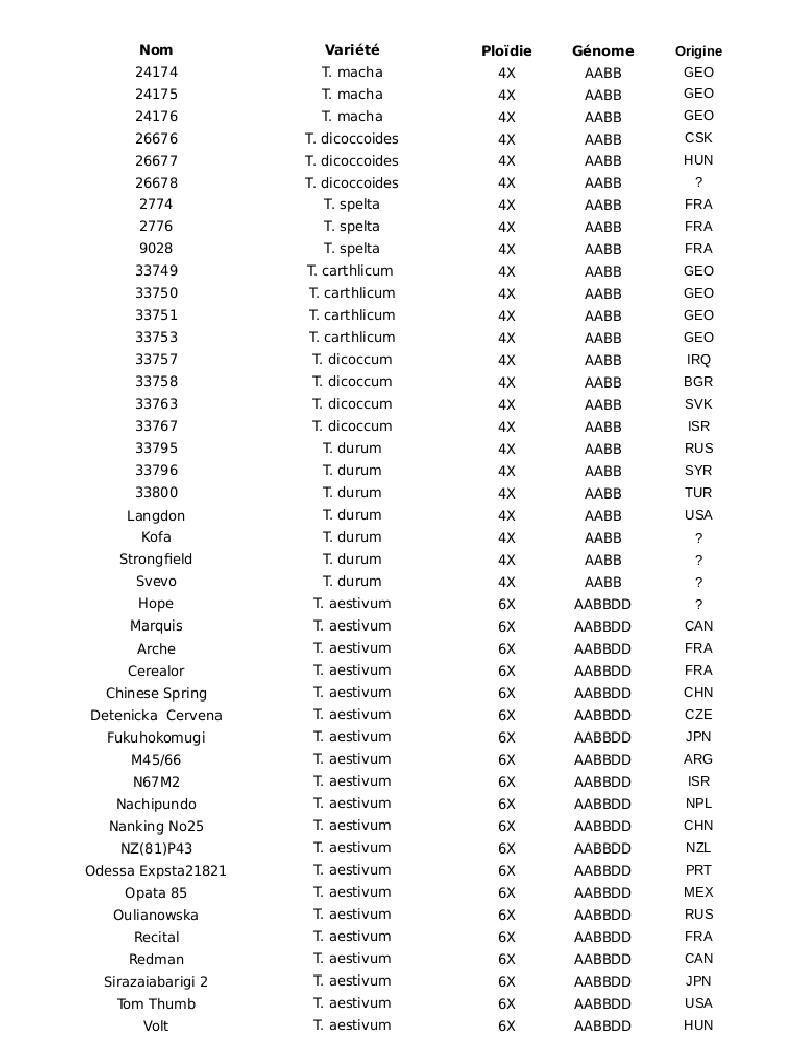
\includegraphics[scale=0.55]{pic_Data/ane1.jpg}\\
\end{center}

Détails des 45 variétés de blé utilisées lors de cette étude. 6 variétés de \textit{Triticum} sont représentées ainsi qu'une origine géographique variée. Certaines accessions n'ont pas encore de nom générique du fait qu'elles ne soient pas commercialisées.

L'origine géographique indiquée correspond au pays où le croisement ayant permis d'acquérir cette variété a été effectué.

\newpage
\begin{center}
\Large\textbf{Annexe 2}\\
\vspace{1cm}
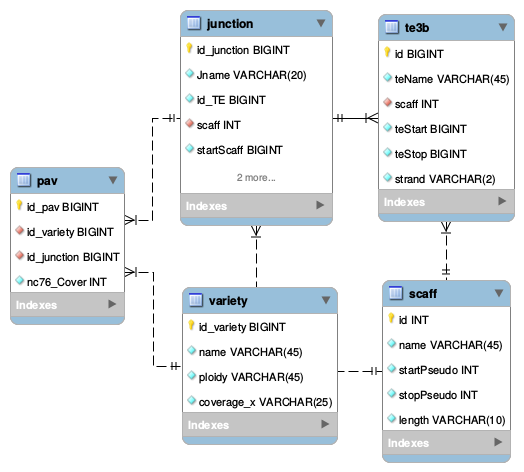
\includegraphics[scale=0.75]{pic_Data/ane3.png}\\
\end{center}

Diagramme de la structure de la base de donnée (BDD) mySQL utilisée afin de stocker les données de présence ou d'absence des marqueurs ISBP entre le chromosome 3B de \textit{Chinese Spring} et celui de 44 autres accessions de blé.

La table \bsc{pav} (Presence-Absence Variation) assigne à chaque id\_pav unique une id\_variety (45 possibles, 44 accessions + \textit{Chinese Spring}) et une id\_junction. Le score nc76\_coverage définit la couverture (nombre de lectures de séquençage alignées) sur le nucléotide \No 76 représentant la jonction.

Les tables \bsc{scaff} et \bsc{te3b} permettent de repositionner les marqueurs sur les ET dont ils sont issus et dans les scaffolds le long du chromosome 3B.

Les données en majuscule suivant les noms de champs de tables indiquent le type de données stockées (BIGINT/INT: entier naturel, VARCHAR(): chaîne de caractères alphanumériques).\\

\newpage
\begin{center}
\Large\textbf{Annexe 3}\\
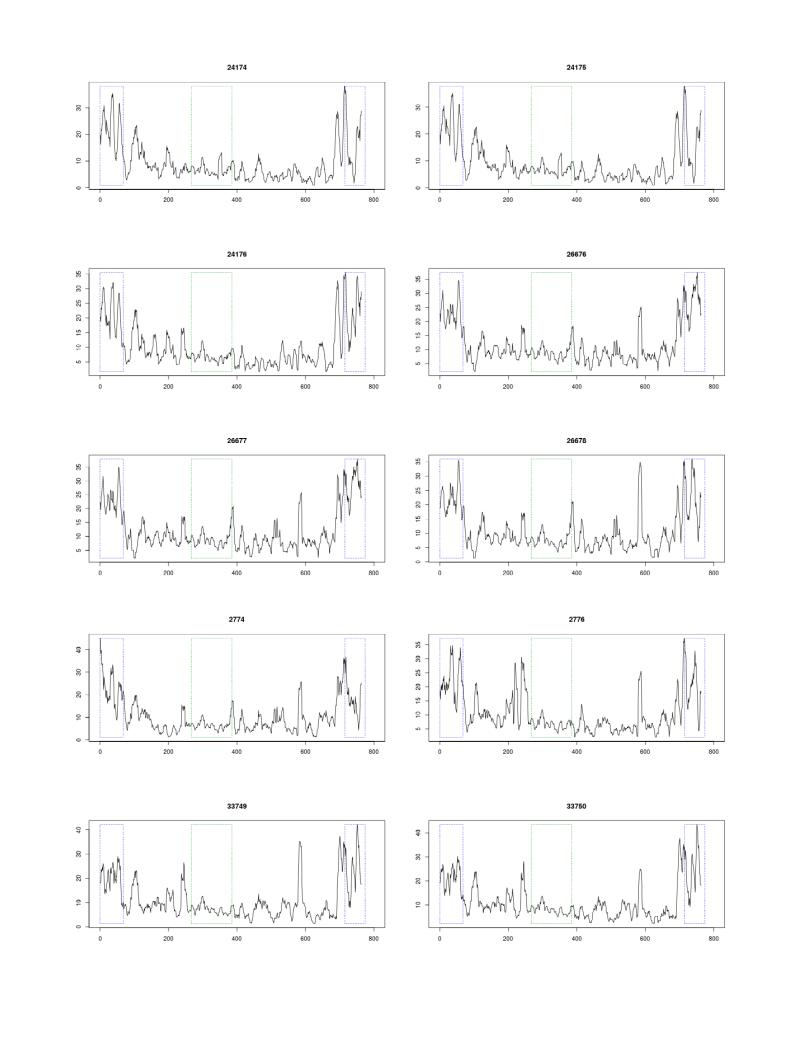
\includegraphics[scale=0.64]{pic_Data/ane2-1.jpg}\\
\thispagestyle{empty}
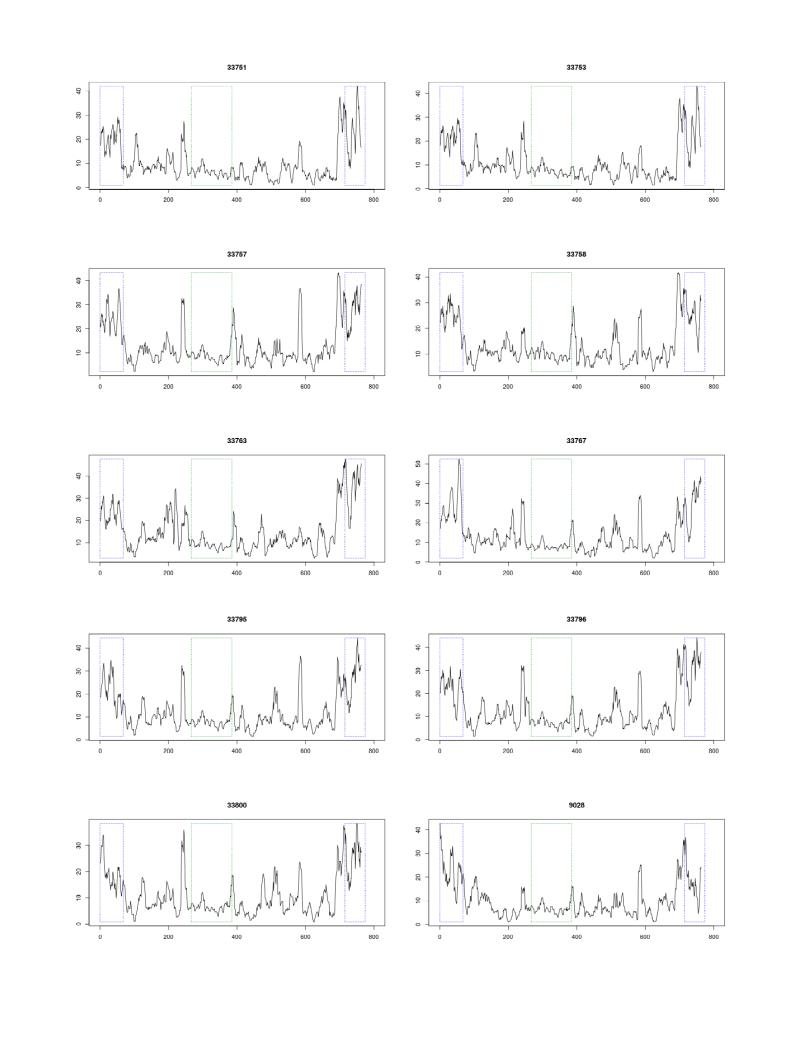
\includegraphics[scale=0.64]{pic_Data/ane2-2.jpg}\\
\thispagestyle{empty}
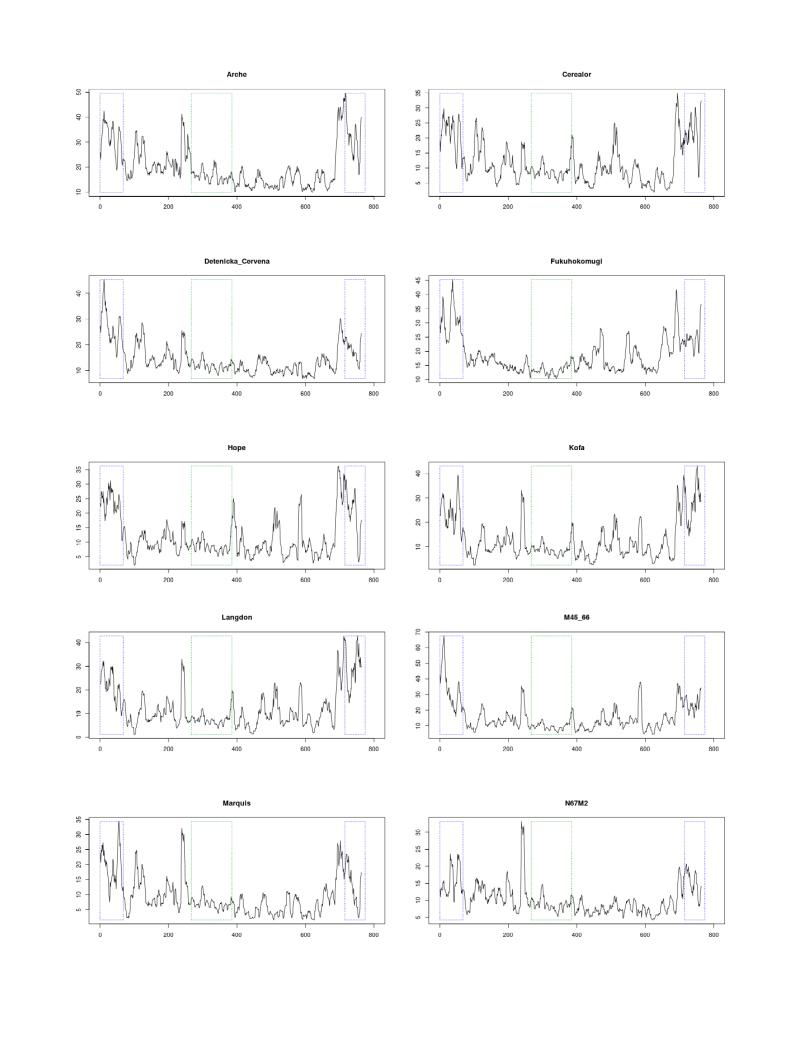
\includegraphics[scale=0.64]{pic_Data/ane2-3.jpg}\\
\thispagestyle{empty}
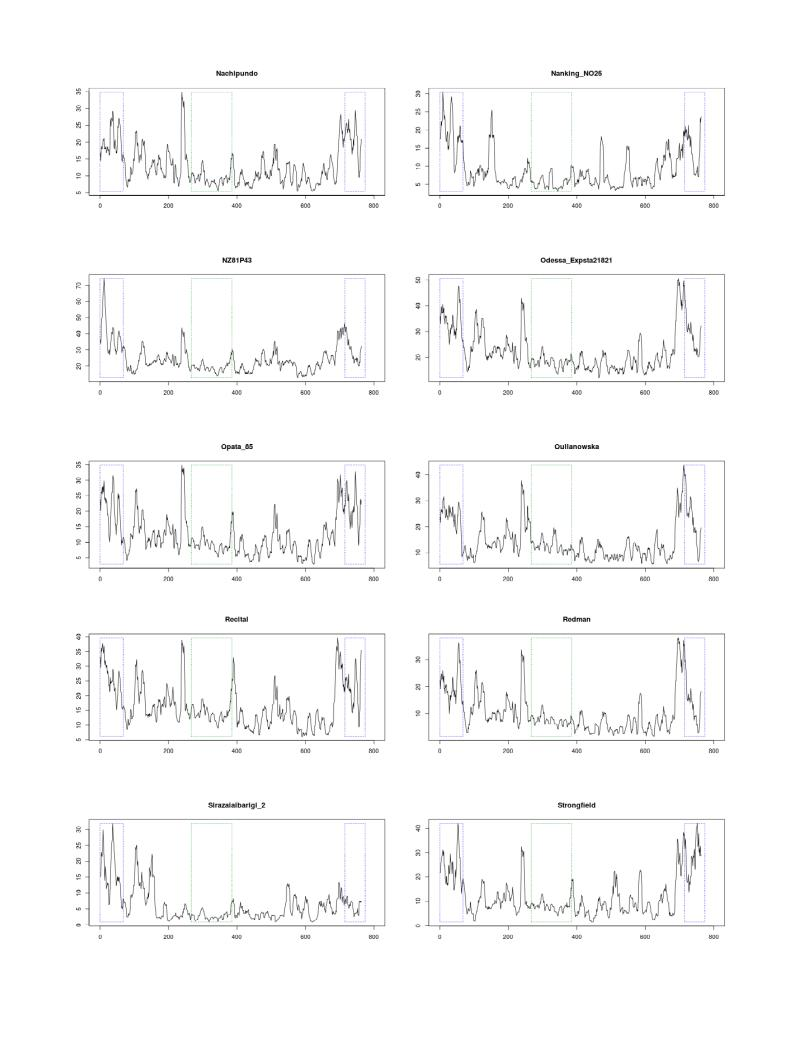
\includegraphics[scale=0.64]{pic_Data/ane2-4.jpg}\\
\thispagestyle{empty}
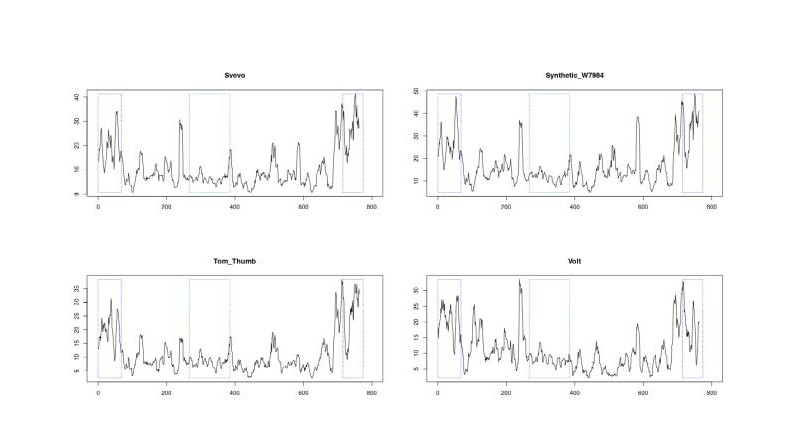
\includegraphics[scale=0.64]{pic_Data/ane2-5.jpg}\\
\thispagestyle{empty}
\end{center}

Pourcentage local de marqueurs ISBP polymorphes (en ordonnée) entre la variété étudiée et  \textit{Chinese Spring} le long du chromosome 3B (en abcisse, en Mb). Pour chaque variété, on remarque que les zones télomériques (cadres bleus) comportent beaucoup plus de marqueurs polymorphes que la zone péricentromérique (cadre vert). Des pics de forte variabilité encadrent cette zone plus conservée.\\

\newpage
\thispagestyle{empty}

\begin{center}
\Large\textbf{Annexe 4}\\
\end{center}

\definecolor{darkGreen}{rgb}{0,0.30,0}
\lstset{language=Perl, breaklines=true, commentstyle=\color{darkGreen}\textbf, tabsize=1, basicstyle=\tiny}
\begin{lstlisting}[frame=single]
#!/share/apps/bin/perl

### Import packages used by the programm.
use strict;
use warnings;
use Getopt::Long;
use DBD::mysql;
use Data::Dumper;
use File::Basename;
use vars qw($help $output $out_log);
use Bio::SeqIO;
use Bio::Tools::GFF;
use Bio::SeqFeature::Generic;
use Bio::Location::Split;
use Bio::SearchIO;

### Define program's options.
my $VERSION = '2.1';
my $lastmodif = '2014/06/28';
my $time = localtime;
my $userName = 'root';
my $password = '********';
my $hostName = 'localhost';
my $port = 3306;
my $dbName = '3b';
my $output;
my $outLog;

&GetOptions ( "h|help"           => \&help,
              "u|username=s"     => \$userName,
              "p|password=s"     => \$password,
              "host=s"           => \$hostName,
              "d|dbname=s"       => \$dbName,
              "o"                => \$output,
              "l"                => \$outLog );

@ARGV or &help;
&main(\@ARGV);

### This program work by passing through different subroutines, this is the main sub.
sub main {
	my $self = {};
	bless $self;
	$self->{inputFiles} = shift;
	$self->setOptions();
	$self->connectToDB();
	$self->startLog() if ($self->{outLog});
	foreach (@{$self->{inputFiles}}){
		$self->{currentFile} = $_;
		unless (-e $self->{currentFile}) {
			print STDERR "*** Could not find " . $self->{currentFile} . " ***\n";
			next;
		}
		$self->readFile();
	}
	$self->{dbi}->disconnect();
	exit(0);
}

### This sub allow the programm to assign variables as options.
sub setOptions {
	my $self = shift;
	$self->{userName} = $userName;
	$self->{hostName} = $hostName;
	$self->{password} = $password;
	$self->{port} = $port;
	$self->{dbName} = $dbName;
	$self->{output} = $output;
	$self->{outLog} = $outLog;
	$self->{log}->{time} = $time;
	return 1;
}

### Sub used to connect mySQL database (containing all TE infos).
sub connectToDB {
	my $self = shift;
	$self->{dbi} = DBI->connect("DBI:mysql:database=" . $self->{dbName} . ";host=" . $self->{hostName}, $self->{userName}, $self->{password})
	                            or die("Could not connect to database" . "\n" . DBI->errstr);
	return 1;
}

### Put log's file values at zero.
sub startLog {
	my $self = shift;
	$self->{log}->{noTE} = 0 ;
	$self->{log}->{"oneTE"} = 0 ;
	$self->{log}->{"multiTE"} = 0 ;
	$self->{log}->{"TEtot"} = 0 ;
	$self->{log}->{"smallTE"} = 0 ;
	$self->{log}->{"junctionTOT"} = 0 ;
	$self->{log}->{"junctionOK"} = 0 ;
	$self->{log}->{"junctionN"} = 0 ;
	$self->{log}->{"junctionOV"} = 0 ;
	$self->{log}->{"st_spNeg"} = 0 ;
	return 1;
}

### Open file containing reference FASTA sequences.
sub readFile {
	my $self = shift;
	$self->{seqIoObj} = Bio::SeqIO->new(-format => "fasta", 
	                                    -file => $self->{currentFile});
	if($self->{output}){
		$self->{outSeqIoObj} = Bio::SeqIO->new(-format => "fasta", 
		                                       -file => ">" . $self->{currentFile} . ".junctions.fna");
	}
	else{
		$self->{outSeqIoObj} = Bio::SeqIO->new(-format => "fasta", 
		                                       -fh => \*STDOUT);
	}
	$self->{log}->{countScaff}=0;
	while ( $self->{seqObj} = $self->{seqIoObj}->next_seq() ) {
		$self->{log}->{countScaff}++;
		$self->{scaffId} = $self->{seqObj}->display_id();
	}
		print STDERR "# " . $self->{scaffId} . "\n";
		
		### mySQL request.
		$self->{sql} = 	"SELECT id," . 
		                       "TEid," .
		                       "start," .
		                       "stop," . 
		                       "start-75 AS st5," . 
		                       "start+75 AS sp5," .
		                       "stop-75 AS st3," .
		                       "stop+75 AS sp3," .
		                       "scaff" .
		                 "FROM annotTE3b" .   
		                 "WHERE scaff='" . $self->{scaffId} . "'" .
		                 "ORDER BY start" ;

		### Execute mySQL request.
		$self->{sth} = $self->{dbi}->prepare($self->{sql});
		$self->{sth}->execute();
		undef $self->{junction};
		while(my $row = $self->{sth}->fetchrow_hashref){
			if ($row->{stop}-$row->{start}+1 < 75){
				$self->{log}->{"smallTE"}++;
				next;
			}
			$self->{junction}->{$self->{scaffId}}->{$row->{id}.'_5'}->{idTe}  = $row->{id}; 
			$self->{junction}->{$self->{scaffId}}->{$row->{id}.'_5'}->{scaff} = $row->{scaff}; 
			$self->{junction}->{$self->{scaffId}}->{$row->{id}.'_5'}->{start} = $row->{st5}; 
			$self->{junction}->{$self->{scaffId}}->{$row->{id}.'_5'}->{stop}  = $row->{sp5}; 

			$self->{junction}->{$self->{scaffId}}->{$row->{id}.'_3'}->{idTe}  = $row->{id}; 
			$self->{junction}->{$self->{scaffId}}->{$row->{id}.'_3'}->{scaff} = $row->{scaff}; 
			$self->{junction}->{$self->{scaffId}}->{$row->{id}.'_3'}->{start} = $row->{st3}; 
			$self->{junction}->{$self->{scaffId}}->{$row->{id}.'_3'}->{stop}  = $row->{sp3}; 
		}

		### Total junctions number in scaffold analysed.
		$self->{log}->{"TEtot"} = scalar(keys(%{$self->{junction}->{$self->{scaffId}}}));
		
		### Count TE number per scaffold (0, 1, several)
		if    ($self->{log}->{TEtot} == 0) { $self->{log}->{"noTE"}++; }
		elsif ($self->{log}->{TEtot} == 1) { $self->{log}->{"oneTE"}++; }
		else                               { $self->{log}->{"multiTE"}++; }
		
		### Define $junction as scaff's key
		print STDERR "->filterOverlappingJunctions\n";
		$self->filterOverlappingJunctions();
		print STDERR "->getSeq\n";
		$self->getSeqOfJunctions();
		print STDERR "->printLog\n";
		$self->printLog() if($self->{outLog});
	}
} 

sub filterOverlappingJunctions {
	my $self = shift;
	my $kRef = 0; 
	REF:foreach my $idRef (sort {$self->{junction}->{$self->{scaffId}}->{$a}->{start} <=> 
	                             $self->{junction}->{$self->{scaffId}}->{$b}->{start}} 
						   keys(%{$self->{junction}->{$self->{scaffId}}})){
		### In case this junction has been discarded based on overlap.
		if($self->{result}->{$self->{scaffId}}->{discard}->{$idRef}) {
			next;
		}
		if ($self->{junction}->{$self->{scaffId}}->{$idRef}->{start} <= 0){
			$self->{result}->{$self->{scaffId}}->{discard}->{$idRef}='startOfScaff';
			next;
		}
		elsif ($self->{junction}->{$self->{scaffId}}->{$idRef}->{stop} > $self->{seqObj}->length){
			$self->{result}->{$self->{scaffId}}->{discard}->{$idRef}='endOfScaff';
			next;
		}

		### Declare refID as "kept" junction before checking for overlapping junctions.
		### Use {start} as value to be able to sort on start in &getSeqOfJunction.
		$self->{result}->{$self->{scaffId}}->{keep}->{$idRef} = $self->{junction}->{$self->{scaffId}}->{$idRef}->{start};
		$kRef++;
		my $startRef = $self->{junction}->{$self->{scaffId}}->{$idRef}->{start};
		my $stopRef = $self->{junction}->{$self->{scaffId}}->{$idRef}->{stop};
		my $kComp = 0;
		COMP:foreach my $idComp (sort {$self->{junction}->{$self->{scaffId}}->{$a}->{start} <=> 
		                               $self->{junction}->{$self->{scaffId}}->{$b}->{start}} 
								keys(%{$self->{junction}->{$self->{scaffId}}})){ 
			my $startComp = $self->{junction}->{$self->{scaffId}}->{$idComp}->{start};
			my $stopComp = $self->{junction}->{$self->{scaffId}}->{$idComp}->{stop};
			
			### Next if same junction ID.
			if ($idRef eq $idComp){next;} 
			
			### Last the foreach loop if start_comp > stop_ref (i.e juction are overlapping).
			if ($startComp > $stopRef){last;}
			
			### Test the overlap.
			if ($startRef<=$stopComp and $startRef>=$startComp){
				$self->{result}->{$self->{scaffId}}->{overlap}->{$idRef}->{++$kComp} = $idComp;
				$self->{result}->{$self->{scaffId}}->{discard}->{$idComp}='overlap';
			}
			elsif ($stopRef<=$stopComp and $stopRef>=$startComp){
				$self->{result}->{$self->{scaffId}}->{overlap}->{$idRef}->{++$kComp}=$idComp;
				$self->{result}->{$self->{scaffId}}->{discard}->{$idComp}='overlap';
			}
		}
	}

	if(scalar(keys%{$self->{result}->{$self->{scaffId}}->{keep}}) + 
       scalar(keys%{$self->{result}->{$self->{scaffId}}->{discard}}) != 
       scalar(keys%{$self->{junction}->{$self->{scaffId}}}) ) {
		die "Error: junctions keep+discard differ from totalNumberOfJunction\n";
	}
	return 1;
}

### Get sequences of junction from fasta files and coordonates from database.
sub getSeqOfJunctions {
	my $self = shift;
	### In $rslt hash, non-overlapping sequences are put inside $subseq.
	foreach my $id ( sort {$self->{result}->{$self->{scaffId}}->{keep}->{$a} <=> 
	                       $self->{result}->{$self->{scaffId}}->{keep}->{$b} }
	                 keys%{$self->{result}->{$self->{scaffId}}->{keep}}){
		my $subseq = $self->{seqObj}->subseq($self->{junction}->{$self->{scaffId}}->{$id}->{start},
		                                     $self->{junction}->{$self->{scaffId}}->{$id}->{stop});
		### No N content test.
		if ($subseq =~/N/i){ 
			$self->{log}->{junctionN}++;
			$self->{result}->{$self->{scaffId}}->{withNs}->{$id}=1;
			next;
		}
		else {
			my $subseqObj = Bio::Seq ->new('-seq' => $subseq, 
			                               '-id' => $id,
			                               '-description' => $self->{scaffId} . "_" . 
			                                                 $self->{junction}->{$self->{scaffId}}->{$id}->{start} . "," .
			                                                 $self->{junction}->{$self->{scaffId}}->{$id}->{stop}); 
			                                
			$self->{log}->{junctionOK}++;
			$self->{result}->{$self->{scaffId}}->{withoutNs}->{$id}=1;
			$self->{outSeqIoObj}->write_seq($subseqObj); 
		}
	}
	return 1;
}

### Print final log to resume the analysis.
sub printLog {
	my $self = shift;

	print join("\t", $self->{scaffId}, "totalNbTE", $self->{log}->{TEtot}), "\n";
	print join("\t", $self->{scaffId}, "totalNbSmallTE", $self->{log}->{smallTE}), "\n";
	print join("\t", $self->{scaffId}, "nbDiscard", scalar keys%{$self->{result}->{$self->{scaffId}}->{discard}}),"\n";
	print join("\t", $self->{scaffId}, "nbKeep", scalar keys%{$self->{result}->{$self->{scaffId}}->{keep}}), "\n";
	print join("\t", $self->{scaffId},  "nbWithNs", scalar keys%{$self->{result}->{$self->{scaffId}}->{withNs}}), "\n";
	print join("\t", $self->{scaffId}, "nbWithoutNs", scalar keys%{$self->{result}->{$self->{scaffId}}->{withoutNs}});

	foreach my $id (sort keys%{$self->{result}->{$self->{scaffId}}->{discard}}){
		print join("\t", $self->{scaffId}, "discardId", $id, $self->{result}->{$self->{scaffId}}->{discard}->{$id}), "\n";
	}
	return 1;
}

### Program's help.
sub help {
my $prog = basename($0);
print STDERR <<EOF ;

# # # $prog # # #
#
# CREATED:    2014/04/22
# LAST MODIF: $lastmodif
# AUTHOR:     Emeric DYNOMANT (INRA Clermont-Ferrand)
# VERSION:    $VERSION
# PURPOSE:    This script is used to design non overlapping junctions 
#             between TE/TE or TE/LowCopyDNA
#             with 75 nt around junctions from annotated mySQL database.
# USAGE:
#             $prog  [OPTIONS]  fastaFile1  fastaFile2  ...
#
# OPTIONS:
#             -h       print this help
#             -l       print details in log file (XLS format)
#             -o       redirect output into a file [default: STDOUT]
#             -u       <string>  sql username [default: root]
#             -p       <string>  sql password [default: ********]
#             -host    <string>  sql hostname [default: localhost]
#             -d       <string>  sql DB name  [default: 3b]

EOF
	exit(1) ;
}
\end{lstlisting}

\vspace{1cm}
Code source du programme \textit{isbpExtract.pl}. Ce programme a été écrit en langage \bsc{perl} afin de dessiner les jonctions aux extrémités des ET le long du chromosome 3B de \textit{Chinese Spring} (marqueurs ISBP) en respectant les contraintes décrites dans la section matériels et méthodes.\\

\thispagestyle{empty}
\end{onehalfspace}
\end{document}